\documentclass[aps,prd,twocolumn,nofootinbib,superscriptaddress,floatfix]{revtex4-2}
\usepackage{graphicx}
\usepackage{amsmath}
\usepackage{siunitx}
\usepackage{booktabs}
\usepackage{placeins}
\usepackage[font=small]{caption}
\usepackage{subcaption}
\usepackage[colorlinks=true,linkcolor=blue,citecolor=blue,urlcolor=blue]{hyperref}
\sisetup{range-phrase=--,range-units=single,separate-uncertainty=true}
\DeclareSIUnit\Gpc{Gpc}
\DeclareSIUnit\Mpc{Mpc}
\setcounter{dbltopnumber}{3}\setcounter{topnumber}{3}\setcounter{totalnumber}{6}
\renewcommand{\dbltopfraction}{0.95}\renewcommand{\topfraction}{0.95}\renewcommand{\textfraction}{0.05}
\renewcommand{\dblfloatpagefraction}{0.75}\renewcommand{\floatpagefraction}{0.75}
\newcommand{\fl}{\ensuremath{\times}}
\begin{document}
\title{Reading the CMB fingerprint of the CoE shell model:\\ what arrangements of masses and voids cancel the leftover residual?}
\author{Chris Alameddin}
\date{October 9, 2026}
\begin{abstract}
In the center-of-explosion (CoE) shell model, the shell's gravity imprints a pattern on the cosmic microwave background around the galactic ring that is 5,751 times the $10^{-5}$ level at which the CMB is flat. Special relativity plus the central mass cancel 95.9\% of it, leaving a residual of 237 times that level. We treat this residual as a fingerprint and pose an inverse problem: which arrangements of added masses and voids cancel it? Using a Newtonian tidal and velocity kernel, we fit compact masses, deep voids, giant partner regions and smooth density fields under several sets of placement rules. Outside our visible sphere, 11 bodies (6 masses and 5 voids) reach the flat target; inside it, 4 to 8 bodies suffice; removing all placement walls brings this to 8. Opening the CoE core completely brings the outside count to 10, but the fits use only its near edge. Sequential, one-at-a-time growth never gets below $27\times$. A smooth field reaches $1\times$ with only about 1\% rms density contrast, but at gigaparsec scales this is roughly $8\sigma$ even against the most generous extrapolation of observed structure. We summarize which solutions exist, how unique they are, and what they would require of the real universe.
\end{abstract}
\maketitle

\section{Introduction}
In the CoE shell model the matter of the universe sits in a thick shell, \SIrange{43.9}{72.5}{\Gpc} from a center of explosion (CoE). We are inside the shell, \SI{58.2}{\Gpc} from the CoE, and our visible universe is a sphere of radius \SI{14.3}{\Gpc} around us (Fig.~\ref{fig:geom}). The visible sphere exactly spans the shell: its near edge touches the inner edge of the shell in the direction of the CoE ($\ell\approx\ang{195}$) and its far edge touches the outer edge in the opposite direction ($\ell\approx\ang{15}$). The us--CoE line is the symmetry axis of the problem. The cosmic microwave background (CMB) we analyze is the ring of sightlines in the galactic plane at the edge of the visible sphere.

\begin{figure*}[t]
\centering
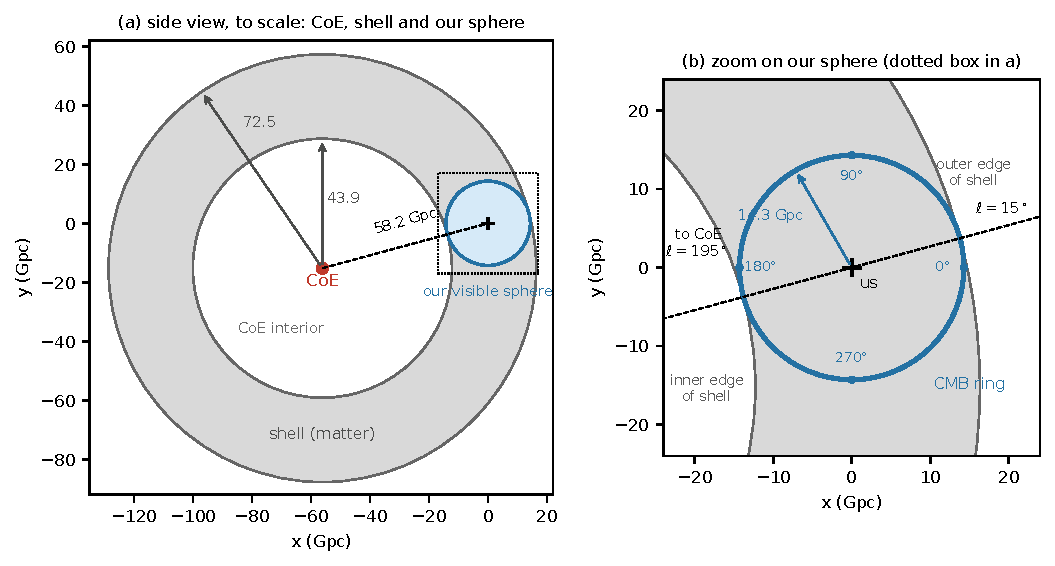
\includegraphics[width=\textwidth]{figures/fig1_geometry.pdf}
\caption{Geometry of the model, side view (looking face-on at the plane of the CMB ring). (a) To scale: the CoE (red), the matter shell (grey, \SIrange{43.9}{72.5}{\Gpc} from the CoE), and our visible sphere (blue, radius \SI{14.3}{\Gpc}) \SI{58.2}{\Gpc} from the CoE. (b) Zoom on our sphere: us ($+$), the CMB ring with galactic longitudes, and the us--CoE axis ($\ell=\ang{195}$ toward the CoE, \ang{15} away). Our sphere just touches both edges of the shell.}
\label{fig:geom}
\end{figure*}

\begin{figure*}[t]
\centering
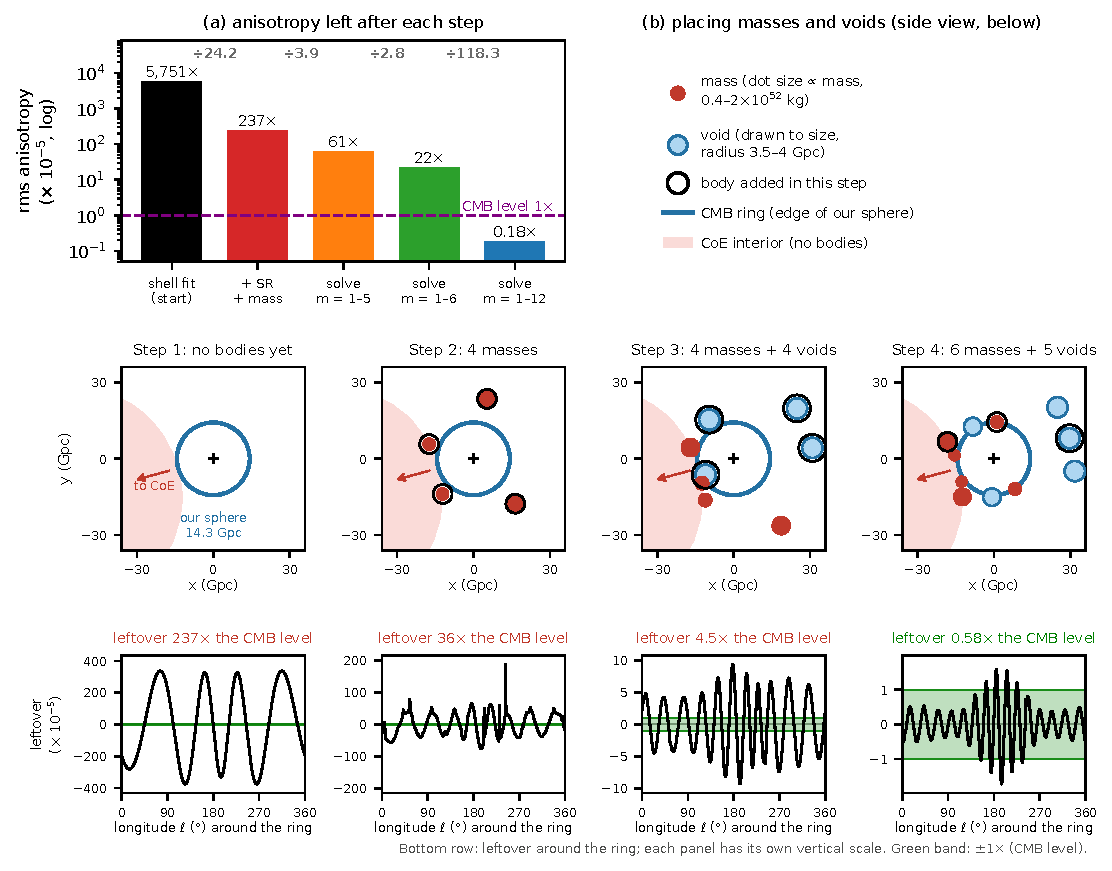
\includegraphics[width=\textwidth]{figures/fig_waterfall.pdf}
\caption{The starting logic, step by step. (a) rms anisotropy around the ring after each step, in units of the $10^{-5}$ CMB level (purple dashed line). The shell alone predicts 5,751\fl; adding special relativity and the central mass brings this to 237\fl, the fingerprint. Solving for its modes $m=1$--5, 1--6 and 1--12 would leave 61\fl, 22\fl\ and 0.18\fl. (b) How placing masses and voids does this, using real fitted layouts outside our sphere (side view: the plane of the CMB ring, seen face-on; bodies are drawn at their position projected onto that plane). Top: the layout; red dots are masses (size grows with mass), blue circles are voids drawn to size, black rings mark the bodies added in that step, and the pink area is the CoE interior, where no body may sit. Bottom: the leftover around the ring, each panel on its own vertical scale; the green band is $\pm1\times$. Step~1: no bodies, 237\fl. Step~2: the best 4 masses, 36\fl. Step~3: the best 4 masses plus 4 voids, 4.5\fl\ (the masses are refitted, so they move). Step~4: 2 masses and 1 void added to step~3 one at a time, refitting all bodies each time (3.0\fl, 1.3\fl, then 0.58\fl), below the CMB level. What remains at step~4 is short waves beyond the solved range, mostly $m=13$--19 (97\% of it).}
\label{fig:waterfall}
\end{figure*}

The logic of this brief starts from Fig.~\ref{fig:waterfall}. On its own, the shell's gravity imprints a strong direction-dependent pattern on the ring: 5,751 times the $10^{-5}$ level at which the CMB is observed to be flat. Our motion relative to the CoE (special relativity: Doppler shift and aberration) and the redshift from the central mass produce a pattern of almost the same shape and opposite sign. Fitting these (speed parameter $\beta_1=0.587$, distance ratio $q=0.230$, mass parameter $\mu=0.0933$, with the axis free; it settles at $\ell=\ang{15.16}$) removes 95.9\% of the starting anisotropy, a reduction by a factor of 24. What is left has an rms of 237 times the floor.

We call this leftover the \emph{fingerprint}. It is a specific shape around the sky, and any structure the model adds must cancel that shape rather than merely reduce its size. The question of this brief is an inverse problem: \emph{what arrangement of masses and voids, placed where, cancels the fingerprint down to the flat target ($1\times$)?} We report every scenario we have run, how many bodies each needs, what the best layouts look like, and how the required structure compares with what is observed.

\section{The fingerprint}
\paragraph*{Gravity against special relativity.} Both large patterns can be broken into waves around the ring. We solve for the residual with modes $m=1$--12, where $m$ counts the number of waves in one full turn and the fingerprint is $R(\ell)=\sum_m c_m\cos m(\ell-\varphi)$ with $\varphi=\ang{15.16}$. Figure~\ref{fig:source} compares, mode by mode, the gravitational multipoles of the shell, $(\ln G)_m$, with the multipoles of special relativity plus the central mass, $(\ln 1/S)_m$. For $m=1$ and 2 they agree to within a few percent and cancel; these modes are where the fit is anchored. For $m=3$--6 they no longer match: at $m=3$ the shell's pattern is about 10\% larger, and from $m=4$ on it falls off faster than the Doppler pattern. This mismatch is what remains. For $m\geq7$ the shell contributes almost nothing and only the tail of the Doppler pattern is left. The difference $c_m=(\ln G)_m-(\ln 1/S)_m$ is the fingerprint (Fig.~\ref{fig:source}b, Table~\ref{tab:modes}).

\paragraph*{The fingerprint mode by mode.} Figure~\ref{fig:fp} draws each mode around the sky. Modes $m=3$, 4 and 5, with amplitudes of 200, 185 and 173 times the floor, carry 92\% of the fingerprint's variance; $m=6$ (81\fl) carries most of the rest. Their sum, a three-lobed shape with an rms of $2.373\times10^{-3}$ (237\fl), is the pattern every scenario below tries to cancel. Modes above 12 are negligible in the fingerprint itself, but they become important once a fit has removed the large ones (Sec.~\ref{sec:examples}).

\begin{figure*}[t]
\centering
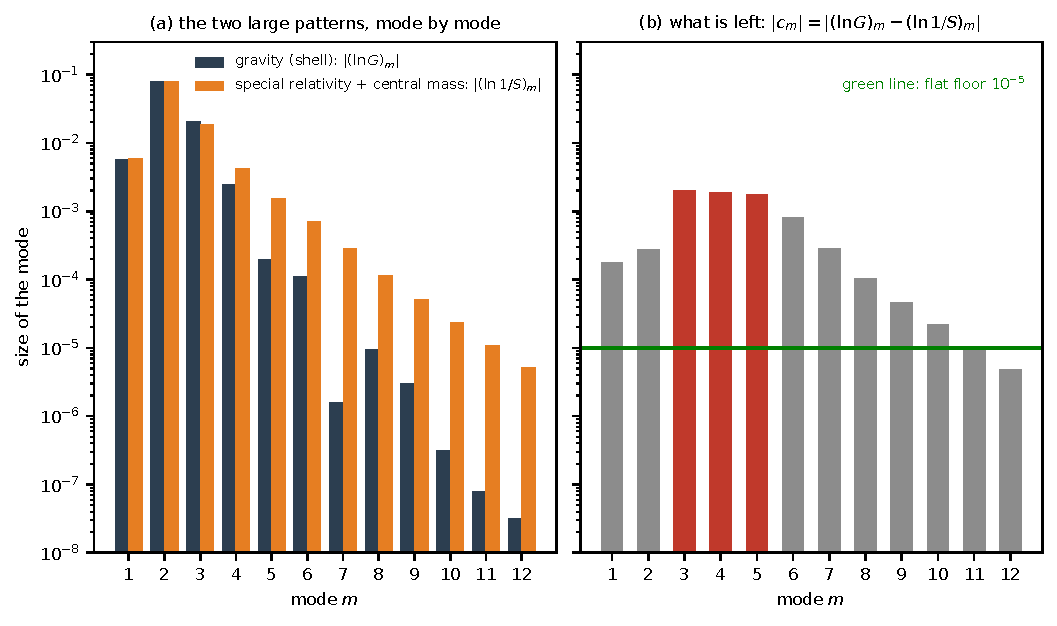
\includegraphics[width=\textwidth]{figures/fig2_source.pdf}
\caption{Where the fingerprint comes from. (a) The size of each mode of the shell's gravitational pattern, $|(\ln G)_m|$ (dark), and of the special-relativity plus central-mass pattern, $|(\ln 1/S)_m|$ (orange), on a log scale. They nearly cancel at $m=1$--2 and part ways from $m=3$ on. (b) What is left, $|c_m|$: the fingerprint, with the big modes $m=3$--5 in red. The green line is the $10^{-5}$ flat level.}
\label{fig:source}
\end{figure*}

\begin{figure*}[p]
\centering
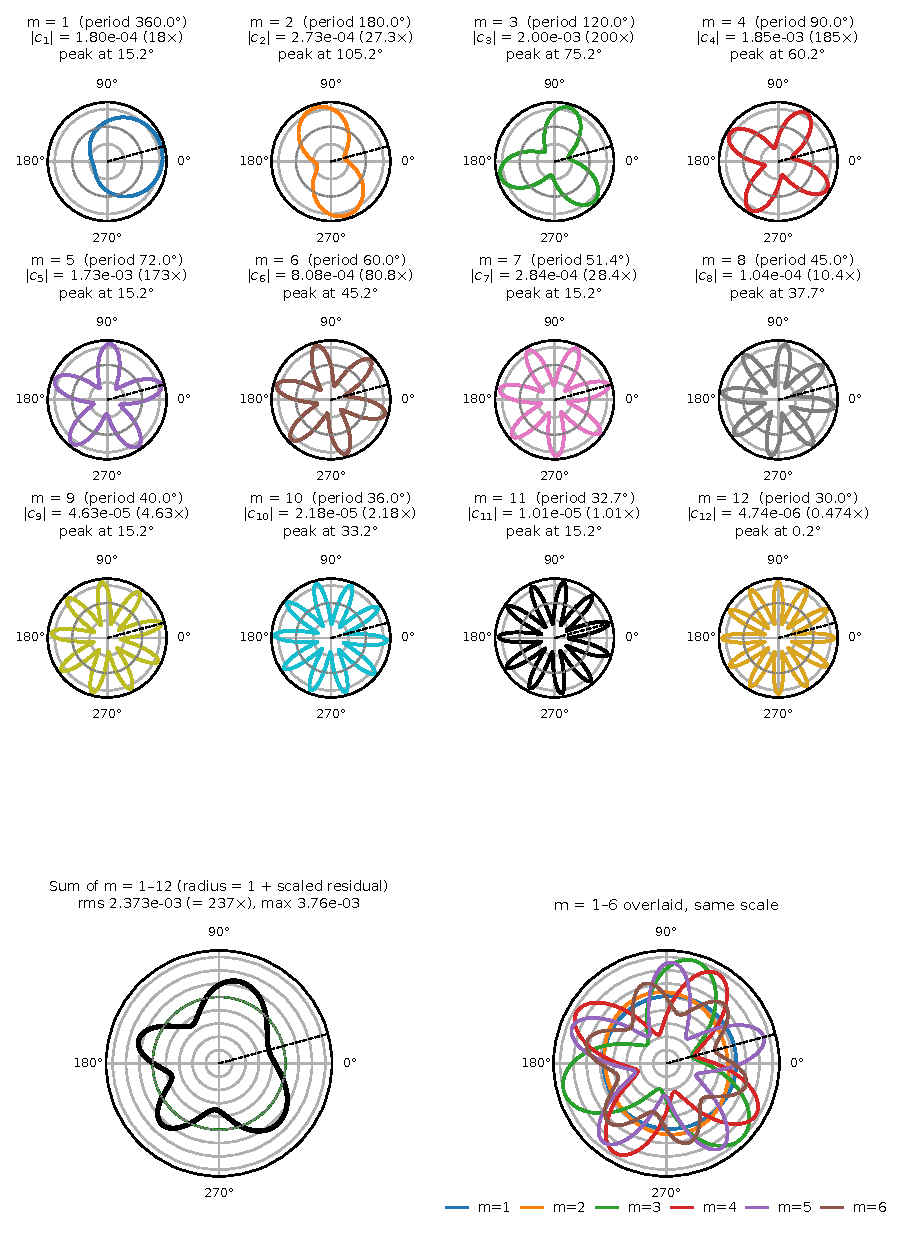
\includegraphics[width=\textwidth,height=0.84\textheight,keepaspectratio]{figures/fig3_modes_polar.pdf}
\caption{The fingerprint: the modes we must solve for. Each small panel draws one mode $c_m\cos m(\ell-\varphi)$ around the sky as radius $=1+$ (scaled mode); the dotted circle is zero and the dashed line is the symmetry axis at $\ell=\ang{15.16}$. Each small panel has its own scale; the numbers give the size, in absolute units and in units of the $10^{-5}$ floor. Bottom left: the sum of $m=1$--12, the full fingerprint; the green circle is the $\pm1\times$ CMB band, thinner than the line at this scale. Bottom right: $m=1$--6 overlaid on one common scale, showing how $m=3$--5 dominate.}
\label{fig:fp}
\end{figure*}

\begin{table*}[tp]
\caption{The modes of the fingerprint. $c_m$: amplitude (absolute and in units of the $10^{-5}$ floor); peak: longitude of the first maximum; \% of var.: share of the fingerprint's variance; $(\ln G)_m$ and $(\ln 1/S)_m$: the shell-gravity and special-relativity plus central-mass multipoles whose difference is $c_m$.}
\label{tab:modes}
\footnotesize
\begin{ruledtabular}
\begin{tabular}{rrrrrrrrl}
$m$ & period (\si{\degree}) & $c_m$ & $|c_m|$ (\fl) & peak (\si{\degree}) & \% of var. & $(\ln G)_m$ shell & $(\ln 1/S)_m$ SR + mass & origin\\
\midrule
1 & 360.0 & $+1.80\times10^{-4}$ & 18 & 15.16 & 0.29 & $-5.68\times10^{-3}$ & $-5.86\times10^{-3}$ & fit matches (cancels)\\
2 & 180.0 & $-2.73\times10^{-4}$ & 27.3 & 105.16 & 0.66 & $+7.81\times10^{-2}$ & $+7.83\times10^{-2}$ & fit matches (cancels)\\
3 & 120.0 & $-2.00\times10^{-3}$ & 200 & 75.16 & 35.56 & $-2.08\times10^{-2}$ & $-1.88\times10^{-2}$ & shell vs Doppler mismatch\\
4 & 90.0 & $-1.85\times10^{-3}$ & 185 & 60.16 & 30.29 & $+2.42\times10^{-3}$ & $+4.27\times10^{-3}$ & shell vs Doppler mismatch\\
5 & 72.0 & $+1.73\times10^{-3}$ & 173 & 15.16 & 26.56 & $+1.96\times10^{-4}$ & $-1.53\times10^{-3}$ & shell vs Doppler mismatch\\
6 & 60.0 & $-8.08\times10^{-4}$ & 80.8 & 45.16 & 5.80 & $-1.13\times10^{-4}$ & $+6.97\times10^{-4}$ & shell vs Doppler mismatch\\
7 & 51.4 & $+2.84\times10^{-4}$ & 28.4 & 15.16 & 0.71 & $+1.56\times10^{-6}$ & $-2.80\times10^{-4}$ & Doppler tail only\\
8 & 45.0 & $-1.04\times10^{-4}$ & 10.4 & 37.66 & 0.10 & $+9.37\times10^{-6}$ & $+1.13\times10^{-4}$ & Doppler tail only\\
9 & 40.0 & $+4.63\times10^{-5}$ & 4.63 & 15.16 & 0.02 & $-3.05\times10^{-6}$ & $-5.02\times10^{-5}$ & Doppler tail only\\
10 & 36.0 & $-2.18\times10^{-5}$ & 2.18 & 33.16 & 0.00 & $+3.10\times10^{-7}$ & $+2.34\times10^{-5}$ & Doppler tail only\\
11 & 32.7 & $+1.01\times10^{-5}$ & 1.01 & 15.16 & 0.00 & $+7.87\times10^{-8}$ & $-1.09\times10^{-5}$ & Doppler tail only\\
12 & 30.0 & $-4.74\times10^{-6}$ & 0.474 & 0.16 & 0.00 & $-3.20\times10^{-8}$ & $+5.17\times10^{-6}$ & Doppler tail only\\

\end{tabular}
\end{ruledtabular}
\end{table*}

\section{Method}
\paragraph*{Geometry and density.} We are at the origin. The CMB ring is the set of 360 in-plane sightlines at radius $R_\mathrm{vis}=\SI{14.3}{\Gpc}$, one per degree of galactic longitude $\ell$. The CoE lies at $(-56.17,-15.22,0)\,\si{\Gpc}$, \SI{58.2}{\Gpc} from us, in the direction $\ell\approx\ang{195}$. The shell spans \SIrange{43.9}{72.5}{\Gpc} from the CoE. The matter density depends on the distance $r$ from the CoE as
\begin{equation}
\rho(r)=\SI{2.9e-27}{\kilo\gram\per\cubic\meter}\;\exp\!\left[-\frac{r-\SI{58.2}{\Gpc}}{\SI{922.65}{\Gpc}}\right].
\end{equation}

\paragraph*{Kernel.} A body of mass $M$ at position $\mathbf{x}$ changes the signal at ring point $\hat n$ by the line-of-sight difference between its pull at the ring point and its pull on us,
\begin{equation}
\Delta(\hat n)\propto\left[\mathbf{g}_M(R_\mathrm{vis}\hat n)-\mathbf{g}_M(\mathbf{0})\right]\cdot\hat n ,
\end{equation}
with the ring mean removed. This tidal-plus-velocity kernel is plain Newtonian; it is valid for sources inside and outside the ring (checked against an independent calculation for 200 interior positions, correlation $\geq0.99999999$). The \emph{leftover} of a layout is $\mathrm{rms}_\ell(R-\Delta)/10^{-5}$, where $R$ is the starting residual; the start is 237\fl\ and the target is 1\fl.

\paragraph*{Bodies.} \emph{Compact masses} are point masses of \SIrange{e49}{2e52}{\kilo\gram} with a $\delta=+100$ core. \emph{Deep voids} are uncompensated spheres with $\delta=-0.7$ and radius \SIrange{0.5}{4}{\Gpc}. \emph{Shallow voids} follow a compensated profile (mean $\delta\approx-0.35$ inside, compensation out to three radii, net zero) \cite{ClampittJain2015}. \emph{Giant partners} are uniform spheres of radius \SIrange{1}{15}{\Gpc} and $\delta$ between $-0.9$ and $+2$, paired with a uniform contrast $\delta_\mathrm{us}$ of our own sphere.

\paragraph*{Placement rules.} ``Outside'' bodies lie between our sphere and \SI{43}{\Gpc} from us and may not enter the CoE interior (the ``wall''). ``Inside'' bodies lie wholly within our sphere, at least \SI{0.1}{\Gpc} from the ring and clear of us. In the \emph{no-wall} runs the CoE-interior exclusion is removed; its \emph{smooth-density limit} replaces the wall by a mass cap that scales with the local density, $M\le\SI{2e52}{\kilo\gram}\,\rho(\mathbf{x})/\rho(\SI{58.2}{\Gpc})$, and requires each mass to draw its material from a non-overlapping supply sphere $V=M/\rho(\mathbf{x})$. The \emph{all-open} runs also remove the visible-sphere exclusion: bodies may sit anywhere \SIrange{0.5}{43}{\Gpc} from us but may not straddle the ring. Cores never overlap.

\paragraph*{Net mass.} Every fit has zero net mass. Outside fits remove or add the net mass smoothly over the surrounding shell region; inside and all-open fits remove it smoothly over our sphere with the same density shape (whose uniform part produces no signal). We also test no compensation, compensation drawn from outside, and, for partners, strict balance by the partners themselves.

\paragraph*{No-mirror rule.} The problem is nearly symmetric about the plane through us, the CoE and the galactic pole ($\ell\to2\times\ang{15.16}-\ell$), and the best fits use mirror pairs. In the no-mirror runs two bodies of the same kind are forbidden if one lies within \ang{20} of the other's mirror image \emph{and} their distances agree within 15\% \emph{and} their sizes within 25\%; no body may lie within \ang{10} of the mirror plane.

\paragraph*{Fitting.} Each body has four free numbers (distance, longitude, latitude, and mass or radius). All are fitted together by bounded least squares (trust-region reflective) from many random starts: 40--100 per body class outside, 12--40 inside, plus warm starts that add one body to the best $N-1$ layout. Sequential runs instead place one body at a time and never refit earlier ones. Field solutions (Sec.~\ref{sec:fields}) solve a regularized linear inverse problem for a continuous $\delta(\mathbf{x})$.

\section{Results}
\begin{figure*}[tp]
\centering
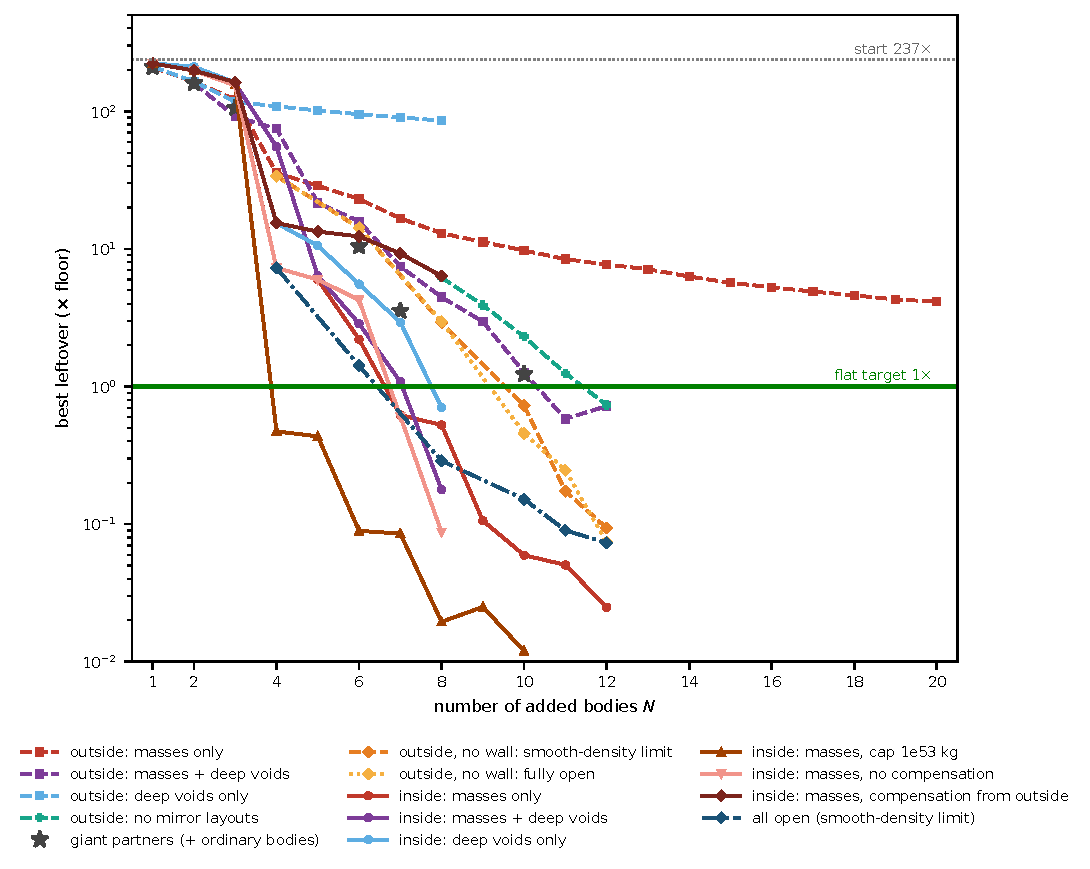
\includegraphics[width=\textwidth]{figures/fig2_overview.pdf}
\caption{Best leftover (in units of the $10^{-5}$ floor, log scale) against the number of added bodies, for all point-body scenarios. Solid lines: inside our sphere; dashed: outside; dash-dot: all open; stars: giant partners. Green: the flat target ($1\times$). Dotted: the start (237\fl).}
\label{fig:overview}
\end{figure*}
\begin{figure*}[tp]
\centering
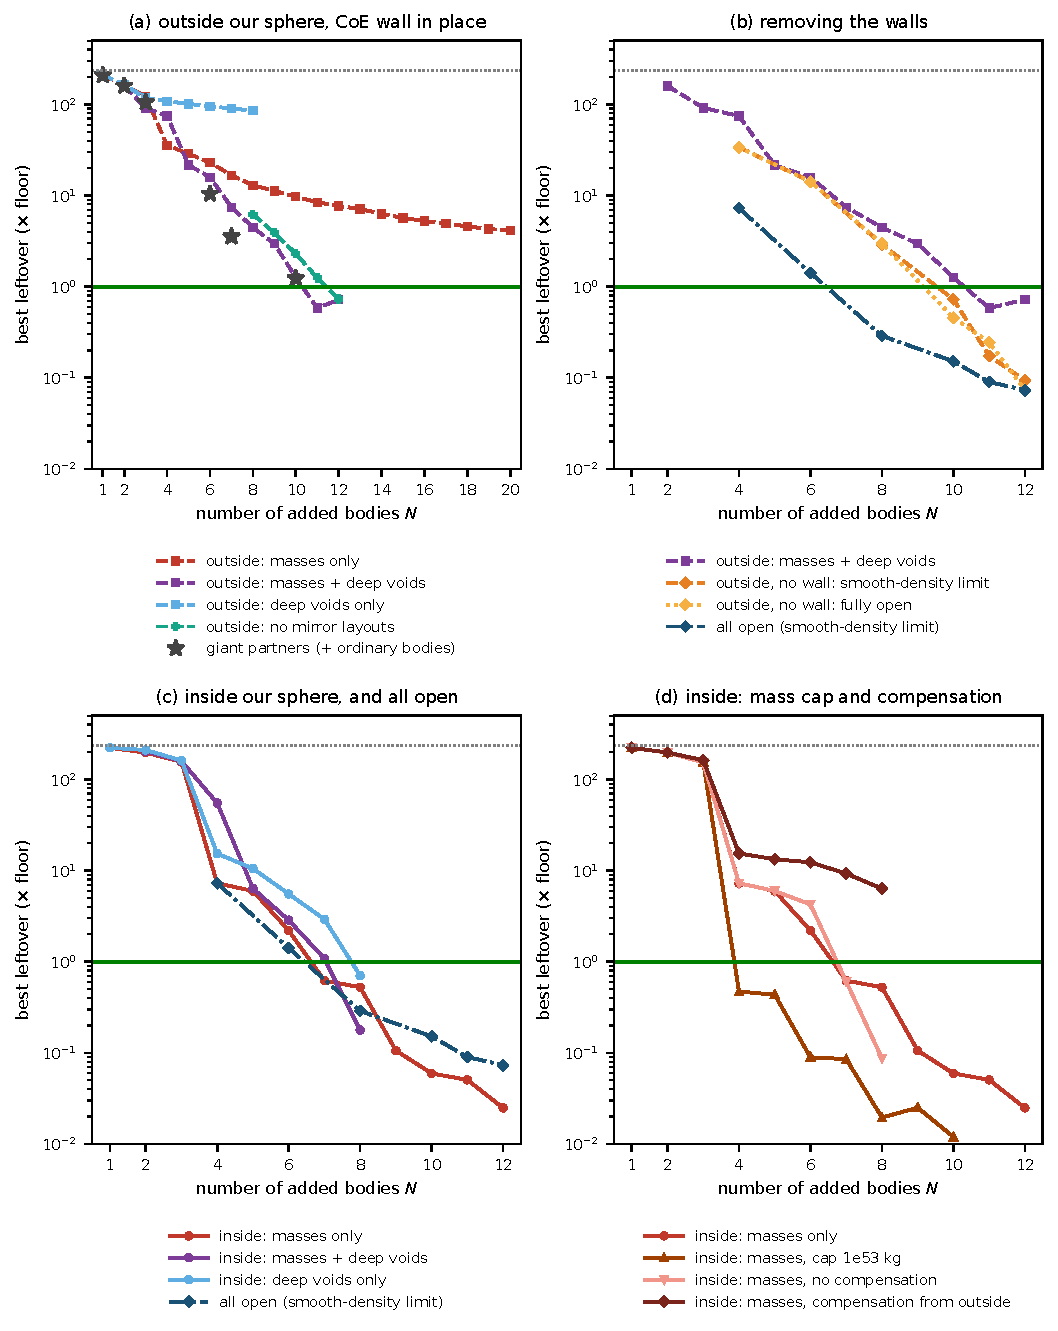
\includegraphics[width=\textwidth]{figures/fig3_families.pdf}
\caption{The same curves by family. (a) Outside our sphere with the CoE wall in place. (b) The effect of removing the CoE wall and then the visible-sphere exclusion. (c) Inside our sphere, compared with all open. (d) Inside variants: a larger mass cap helps most; compensating from outside hurts most.}
\label{fig:families}
\end{figure*}
\begin{table}[tbp]
\caption{Fewest bodies that reach the flat target, and the best value reached (in units of the floor).}
\label{tab:key}
\footnotesize
\begin{ruledtabular}
\begin{tabular}{lcc}
Scenario & first $N<1\times$ & best (at $N$)\\
\midrule
Outside: masses only & -- & 4.14 (20)\\
Outside: masses + deep voids & 11 (0.58) & 0.58 (11)\\
Outside: deep voids only & -- & 85.3 (8)\\
Outside: no-mirror layouts & 12 (0.73) & 0.73 (12)\\
Giant partners + bodies & -- & 1.23 (10)\\
No wall: smooth-density limit & 10 (0.73) & 0.094 (12)\\
No wall: fully open & 10 (0.46) & 0.074 (12)\\
Core open: masses + deep voids & 10 (0.46) & 0.069 (12)\\
Core open: no-mirror layouts & 11 (0.37) & 0.34 (12)\\
Core open: giant partners + bodies & 10 (0.17) & 0.080 (11)\\
Core open: all open & 8 (0.18) & 0.18 (8)\\
All bodies in the core & -- & 143 (12)\\
Inside: masses only & 7 (0.62) & 0.025 (12)\\
Inside: masses + deep voids & 8 (0.18) & 0.18 (8)\\
Inside: deep voids only & 8 (0.70) & 0.70 (8)\\
Inside: masses, cap \SI{e53}{\kilo\gram} & 4 (0.47) & 0.012 (10)\\
Inside: no compensation & 7 (0.61) & 0.087 (8)\\
Inside: compensation from outside & -- & 6.35 (8)\\
All open (smooth limit) & 8 (0.29) & 0.073 (12)\\
Seq.\ A: deep voids + clusters & -- & 27.4 (48)\\
Seq.\ A: shallow voids & -- & 135 (30)\\
Seq.\ B: CMB-aware growth & -- & 37.2\\
Seq.\ B: foam rule & -- & 222\\
Seq.\ B: random & -- & 213\\
Seq.\ B: shallow voids & -- & 163\\
\end{tabular}
\end{ruledtabular}
\end{table}
\begin{figure}[tbp]
\centering
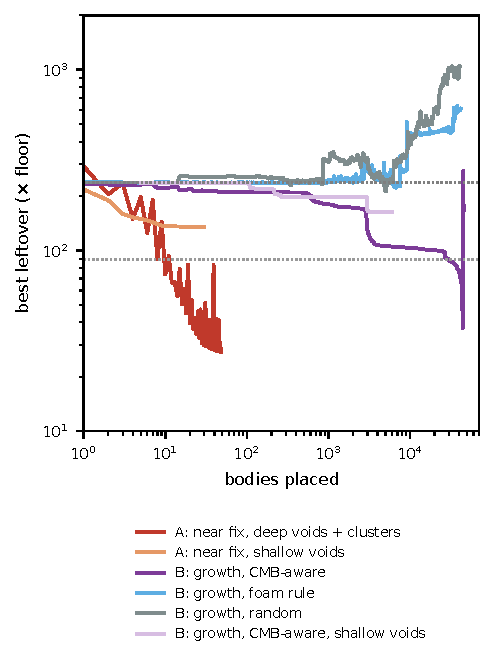
\includegraphics[width=\columnwidth]{figures/fig4_sequential.pdf}
\caption{Sequential placement, one body at a time with no refitting (log scale in bodies placed). A: the near region fixed pair by pair. B: growth from empty until the region is full, under three placement rules. None reaches the flat target (green); the dotted lines mark the start (237\fl) and the four-clump result (89\fl).}
\label{fig:seq}
\end{figure}
\begin{figure*}[p]
\centering
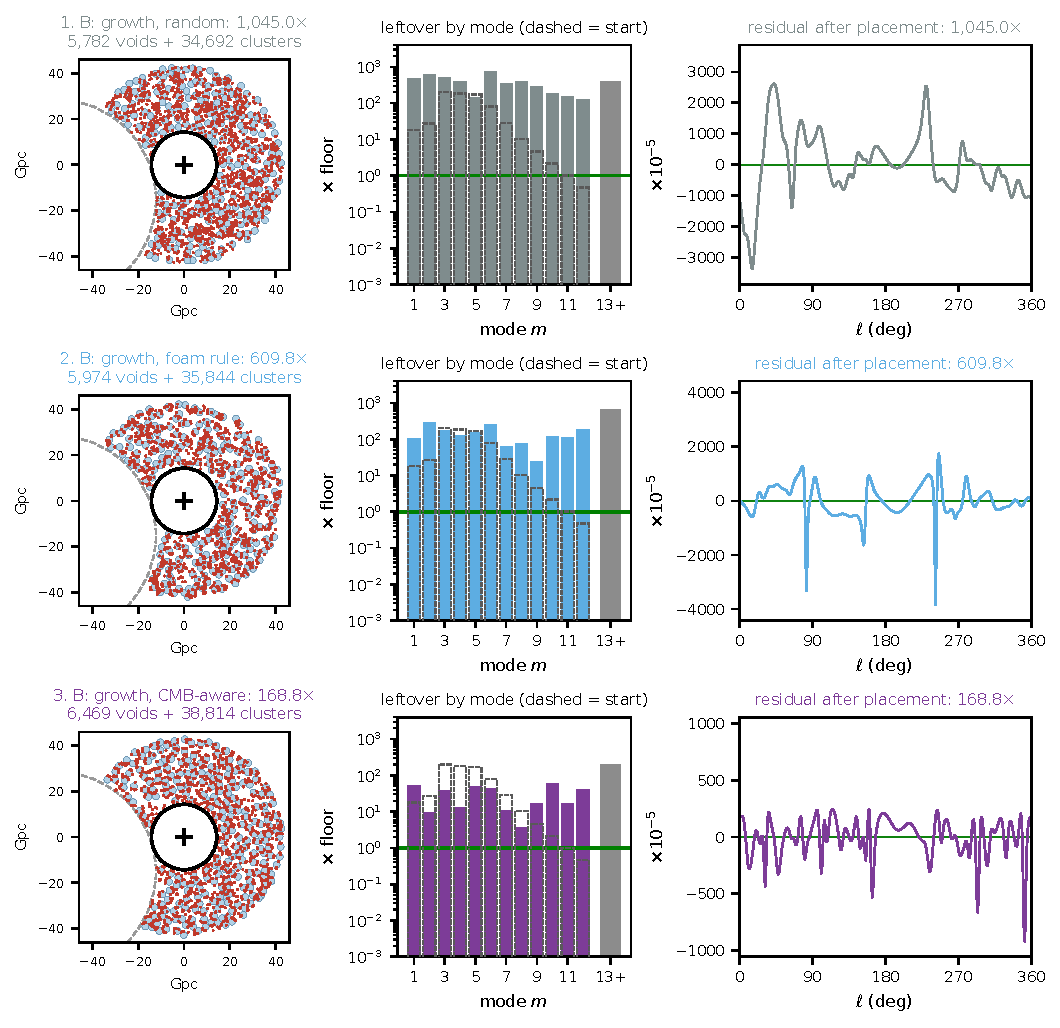
\includegraphics[width=\textwidth]{figures/fig_seq_universes_a.pdf}
\caption{Sequential-placement universes 1--3: the final universe of each curve of Fig.~\ref{fig:seq}. Figures~\ref{fig:sequniv} and \ref{fig:sequniv2} are one sequence of six runs, numbered 1--6 from the largest to the smallest final leftover; each row's titles, bars and residual curve have the colour of its curve in Fig.~\ref{fig:seq}. Left: side view, looking face-on at the plane of the CMB ring (us: $+$; black circle: our \SI{14.3}{\Gpc} sphere and the CMB ring; grey dashed: the CoE-interior wall; blue: voids at their true radius; red dots: clusters). The A runs fill only the near region and all their bodies are shown, projected onto the plane; the B runs fill the whole region out to \SI{42.9}{\Gpc} in three dimensions, so only bodies centred within \SI{1.5}{\Gpc} of the ring plane are drawn. Middle: leftover by mode (dashed outline: start; grey bar: all modes above 12 combined; green: $1\times$). Right: residual around the ring after placement, each on its own vertical scale; the green band is $\pm1\times$. The B layouts were not saved by the original runs and were regenerated with the same code and random seed; they reproduce the saved final leftovers. This figure: 1, B growth with random placement (5,782 voids and 34,692 clusters, 1,045\fl); 2, B growth with the foam rule (5,974 voids and 35,844 clusters, 610\fl); 3, B growth, CMB-aware (6,469 voids and 38,814 clusters, 169\fl).}
\label{fig:sequniv}
\end{figure*}
\begin{figure*}[p]
\centering
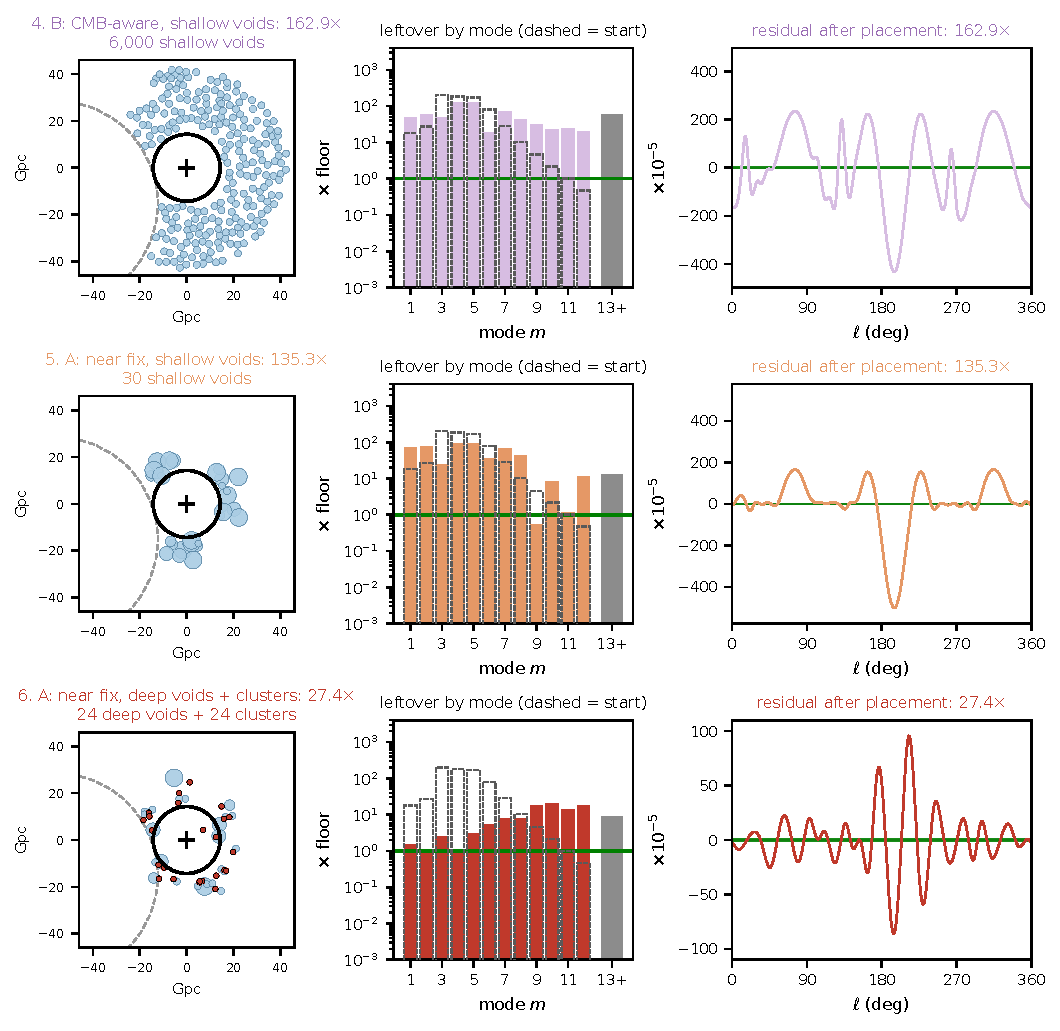
\includegraphics[width=\textwidth]{figures/fig_seq_universes_b.pdf}
\caption{Sequential-placement universes 4--6 of the sequence begun in Fig.~\ref{fig:sequniv} (largest to smallest final leftover; panels as in Fig.~\ref{fig:sequniv}): 4, B growth, CMB-aware, with shallow voids (6,000 voids, 163\fl); 5, A near region fixed first, shallow voids (30 voids, 135\fl); 6, A near region fixed first, deep voids and clusters (24 of each, 27.4\fl; the same layout as example 1 in Fig.~\ref{fig:ex1}).}
\label{fig:sequniv2}
\end{figure*}
\begin{figure*}[p]
\centering
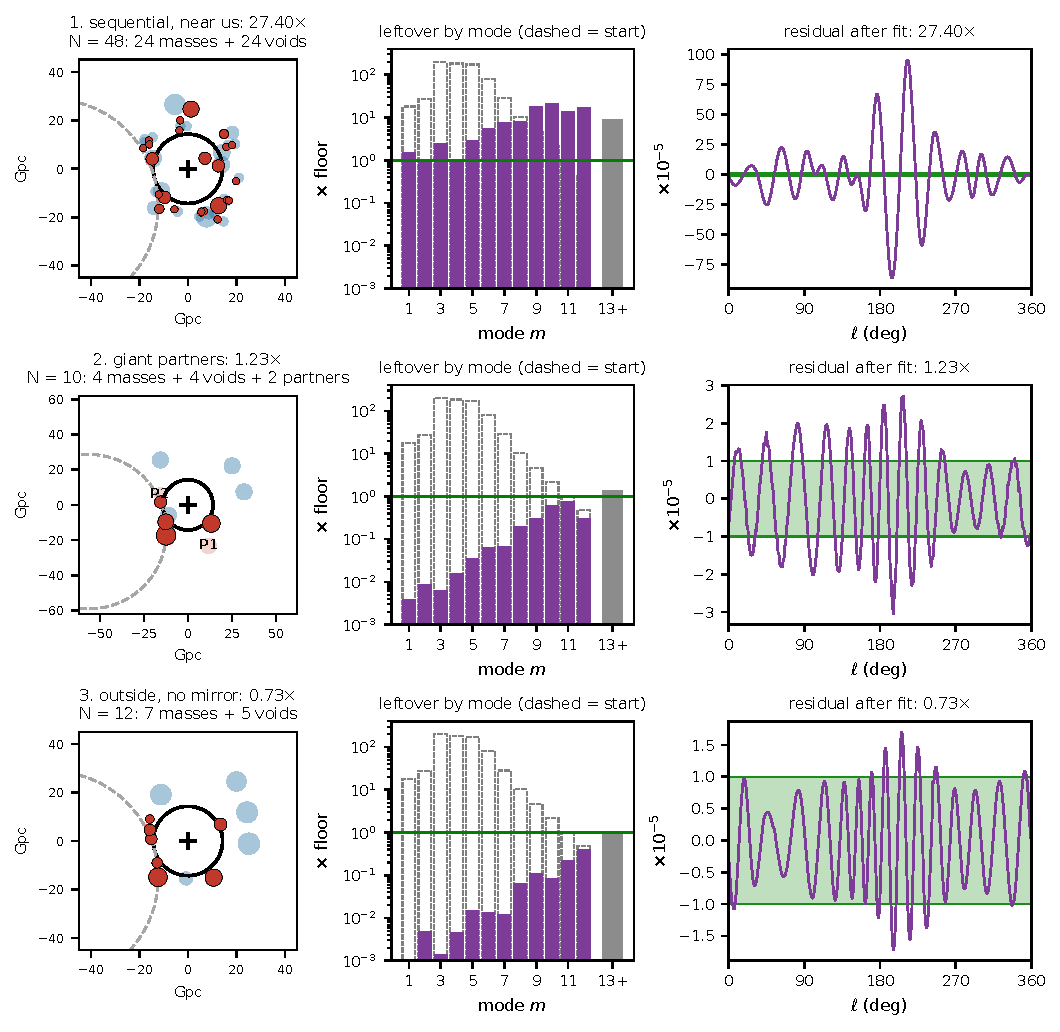
\includegraphics[width=\textwidth]{figures/fig5_examples_outside.pdf}
\caption{Example universes 1--3. Left: side view, looking face-on at the plane of the CMB ring (the galactic plane) (us: $+$; black circle: our \SI{14.3}{\Gpc} sphere; grey dashed: the CoE-interior wall, where it applies; red: masses, sized by mass; blue: voids at their true radius; P1, P2: giant partners; bodies off the plane are projected). Middle: leftover by mode (dashed outline: start; grey bar: all modes above 12 combined; green: $1\times$). Right: residual around the ring after the fit; the green band is $\pm1\times$. Figures~\ref{fig:ex1}--\ref{fig:ex3} are one sequence of nine example universes, numbered 1--9 from the largest to the smallest remaining leftover; Fig.~\ref{fig:ex4} continues with the core-open examples 10--13. This figure: 1, sequential placement in the near region (48 bodies: 24 masses and 24 voids, 27.40\fl), where large residuals remain in every mode; 2, giant partners plus ordinary bodies (10 bodies, 1.23\fl); 3, outside, masses and deep voids with mirror layouts forbidden (12 bodies, 0.73\fl).}
\label{fig:ex1}
\end{figure*}
\begin{figure*}[p]
\centering
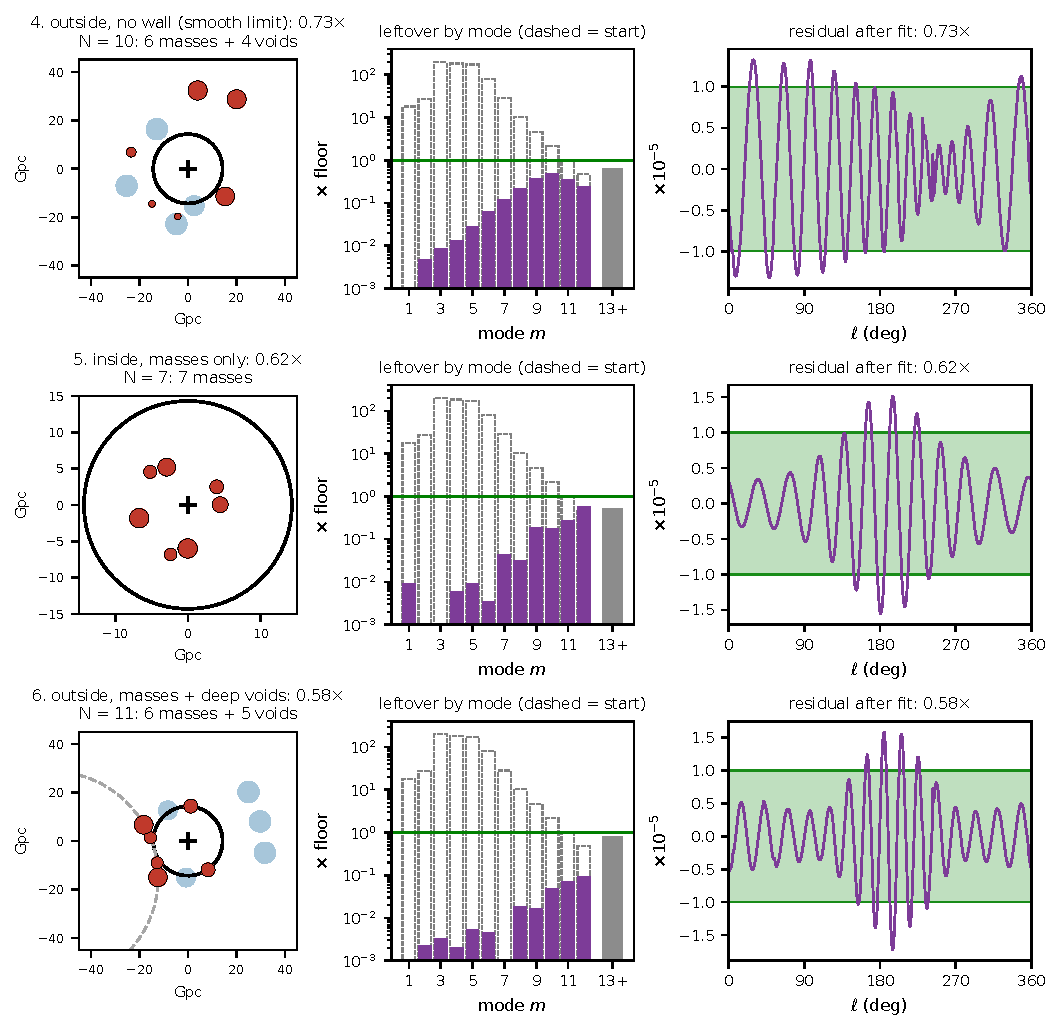
\includegraphics[width=\textwidth]{figures/fig6_examples_open_inside.pdf}
\caption{Examples 4--6 of the sequence begun in Fig.~\ref{fig:ex1} (largest to smallest leftover; panels as in Fig.~\ref{fig:ex1}): 4, outside with no CoE wall and the smooth-density limit (10 bodies, 0.73\fl; 0.726 against 0.734 for example~3); 5, inside our sphere, 7 masses (0.62\fl); 6, outside, masses and deep voids (11 bodies, 0.58\fl).}
\label{fig:ex2}
\end{figure*}
\begin{figure*}[tp]
\centering
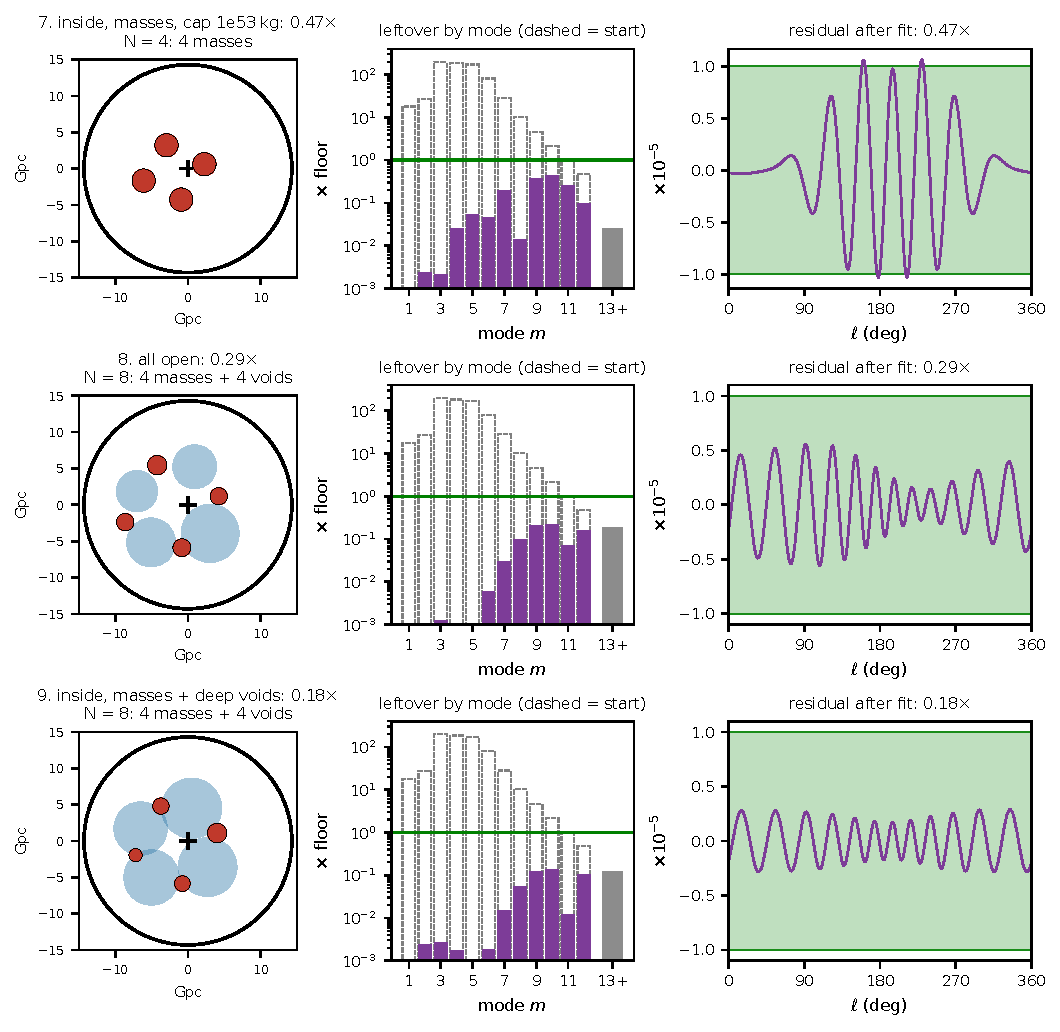
\includegraphics[width=\textwidth]{figures/fig7_examples_more.pdf}
\caption{Examples 7--9 of the sequence begun in Fig.~\ref{fig:ex1} (largest to smallest leftover; panels as in Fig.~\ref{fig:ex1}): 7, inside our sphere, 4 masses with a \SI{e53}{\kilo\gram} cap (0.47\fl); 8, all open, where the eight bodies move inside our sphere (0.29\fl); 9, inside our sphere, 4 masses and 4 voids (0.18\fl).}
\label{fig:ex3}
\end{figure*}
\begin{figure*}[p]
\centering
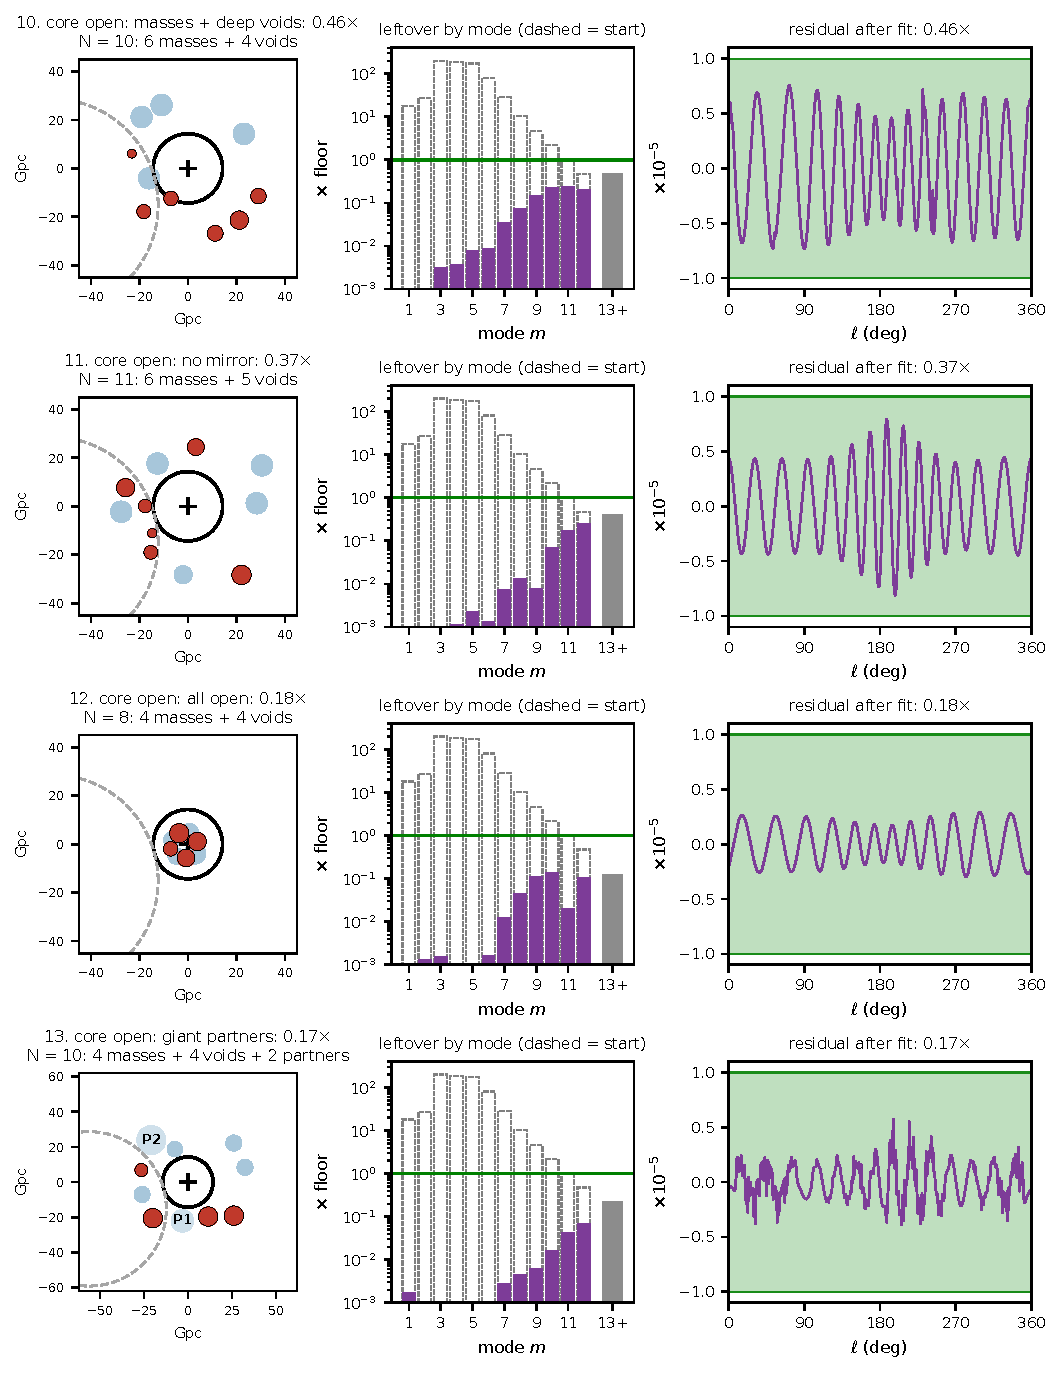
\includegraphics[width=\textwidth,height=0.85\textheight,keepaspectratio]{figures/fig_examples_core_open.pdf}
\caption{Examples 10--13: the same scenarios rerun with the CoE core fully open (Sec.~\ref{sec:coreopen}), at the first $N$ that reaches $1\times$, ordered from the largest to the smallest leftover; panels as in Fig.~\ref{fig:ex1}, and the grey dashed circle is now the edge of the open core rather than a wall. 10, masses and deep voids (10 bodies, 0.46\fl; 3 bodies 1--6\,Gpc inside the core edge); 11, no mirror layouts (11 bodies, 0.37\fl; 5 in the core, 4 of them within 6\,Gpc of the edge); 12, all open (8 bodies, 0.18\fl; none in the core; all eight sit inside our sphere, as in examples 8 and 9); 13, giant partners plus ordinary bodies (10 bodies, 0.17\fl; 3 in the core, 7--13\,Gpc deep).}
\label{fig:ex4}
\end{figure*}
\begin{figure*}[tbp]
\centering
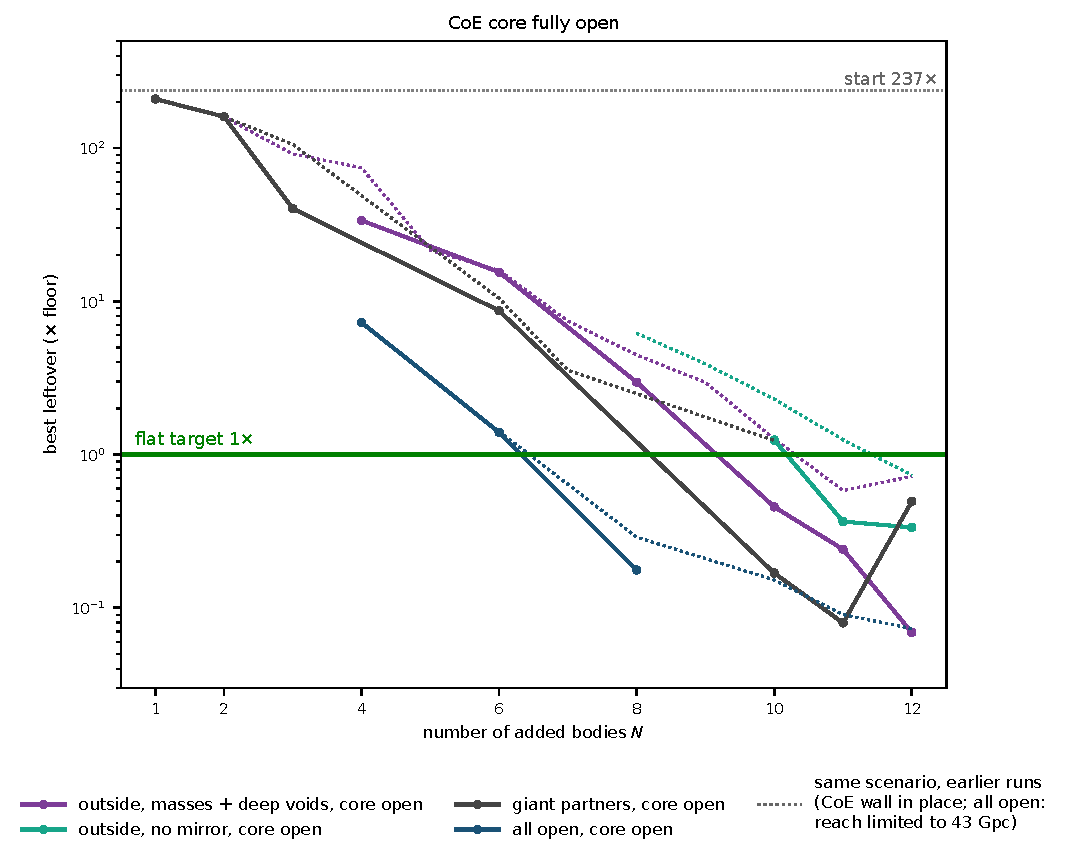
\includegraphics[width=\textwidth]{figures/fig_core_open_best_vs_N.pdf}
\caption{Best leftover against the number of added bodies with the CoE core fully open (solid), compared with the same scenarios in the earlier runs (dotted: CoE wall in place; for all open, reach limited to \SI{43}{\Gpc}). Green: the flat target ($1\times$); dotted grey: the start (237\fl).}
\label{fig:coreopen}
\end{figure*}

\subsection{Leftover versus number of bodies}
Figure~\ref{fig:overview} collects the best leftover against the number of added bodies $N$ for every point-body scenario, and Fig.~\ref{fig:families} splits them into families. Table~\ref{tab:key} lists the first $N$ that reaches the flat target and the best value reached.



Three facts stand out. First, masses alone never reach the target from outside (they stall near 4\fl\ at $N=20$), and voids alone stall near 85\fl; the outside solutions need both, and reach $1\times$ at $N=11$ (6 masses and 5 voids). Second, bodies inside our sphere are far more effective: 7 masses or 4 masses plus 4 voids suffice, and with a looser mass cap of \SI{e53}{\kilo\gram} only 4 masses are needed. Third, each wall that is removed saves bodies: without the CoE-interior wall the target is reached at $N=10$, and with everything open at $N=8$, where all 8 bodies move inside our sphere. Sequential placement (Fig.~\ref{fig:seq}), which never revisits earlier choices, never reaches the target. Figures~\ref{fig:sequniv} and \ref{fig:sequniv2} show the final universe of each sequential run, its leftover by mode and the leftover it leaves around the ring.



\begin{figure*}[tp]
\centering
\begin{subfigure}[b]{0.38\textwidth}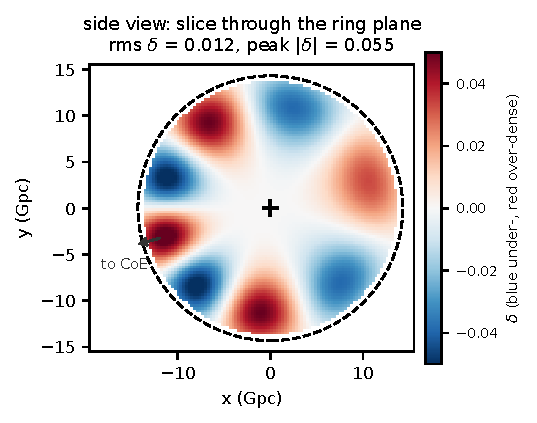
\includegraphics[width=\textwidth]{figures/fig8a_smooth_field_side.pdf}\caption{}\end{subfigure}\hfill
\begin{subfigure}[b]{0.56\textwidth}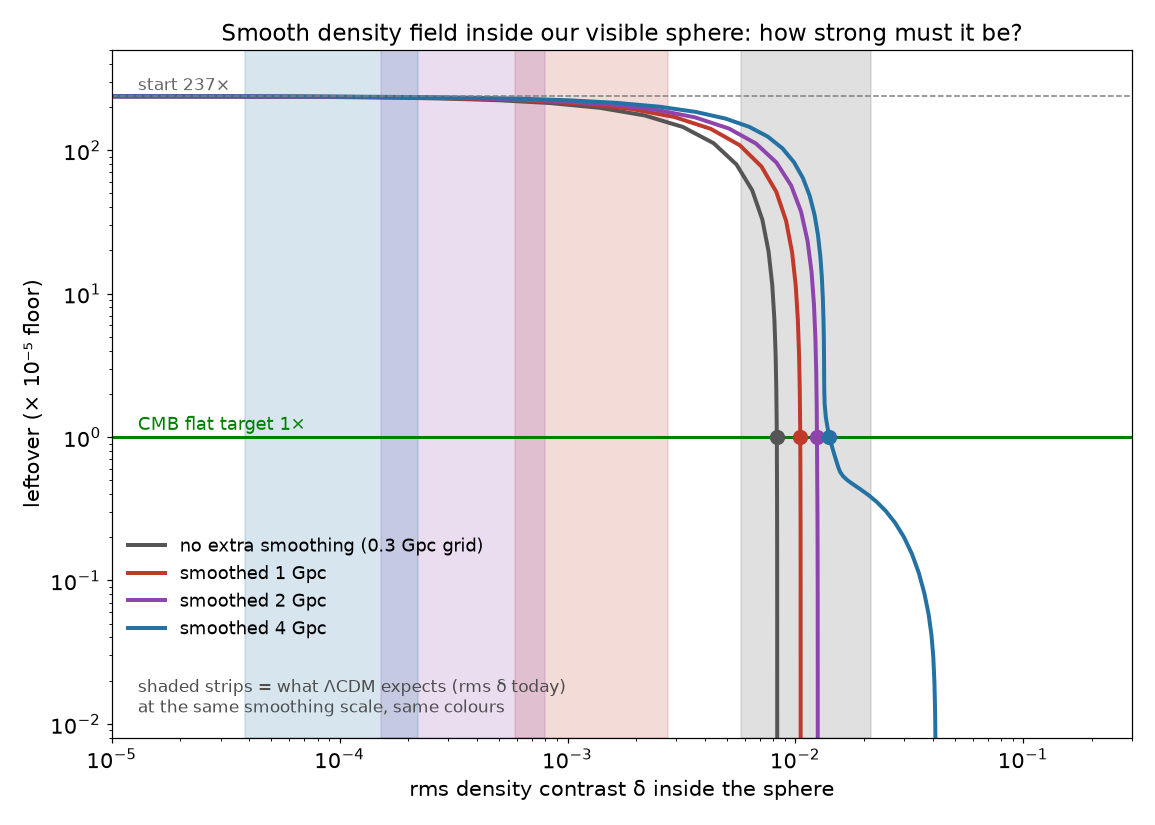
\includegraphics[width=\textwidth]{figures/fig8b_smooth_tradeoff.png}\caption{}\end{subfigure}
\caption{Smooth-field solution. (a) The weakest field that reaches $1\times$ at \SI{2}{\Gpc} smoothing, side view: a slice through the ring plane (red: overdense, blue: underdense; dashed: our \SI{14.3}{\Gpc} sphere). (b) Leftover against the rms density contrast of the field for several smoothing scales; shaded strips mark what standard cosmology expects at the same scales.}
\label{fig:smooth}
\end{figure*}
\begin{figure*}[tp]
\centering
\begin{subfigure}[b]{0.52\textwidth}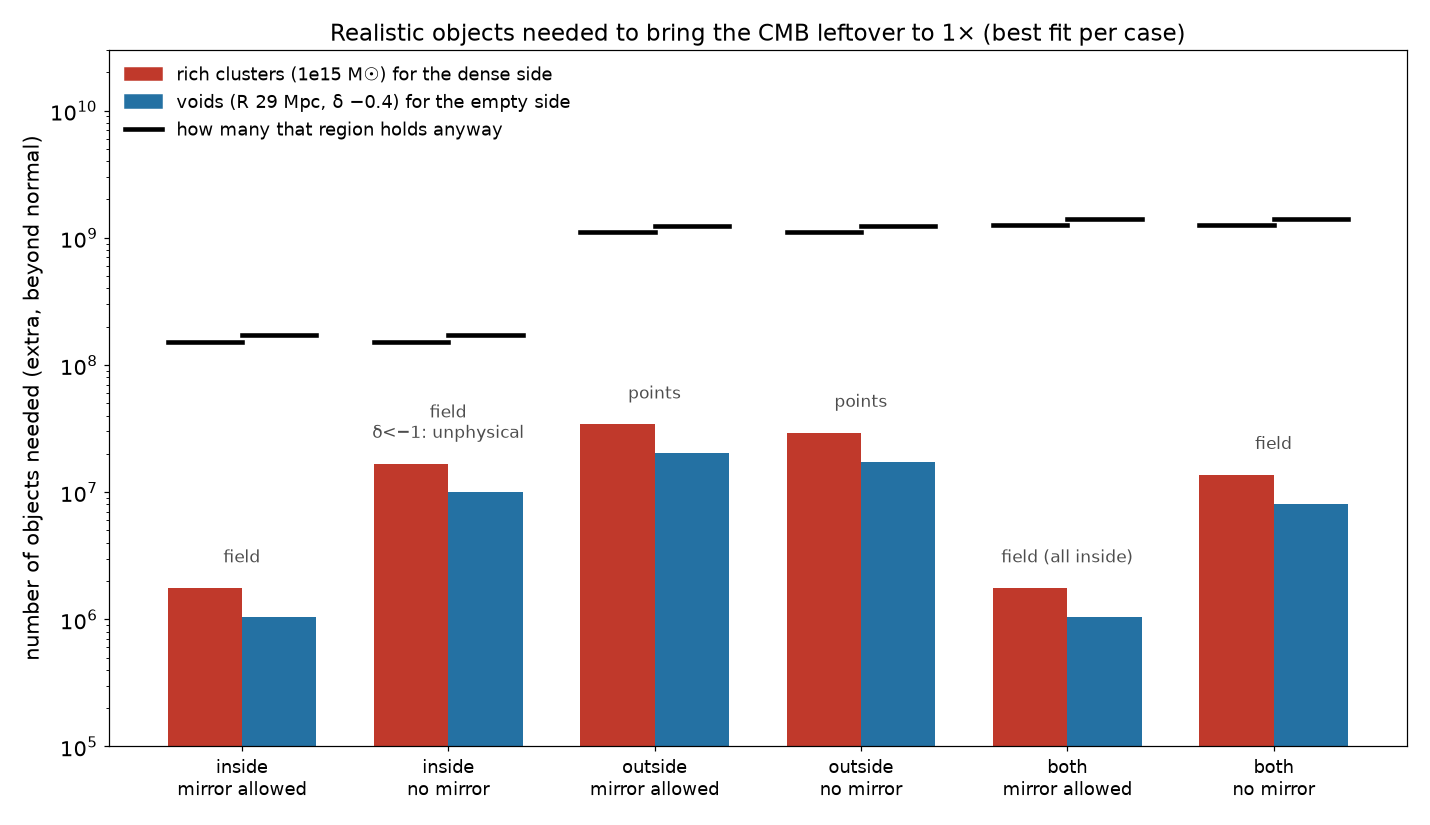
\includegraphics[width=\textwidth]{figures/fig9a_realistic_counts.png}\caption{}\end{subfigure}\hfill
\begin{subfigure}[b]{0.46\textwidth}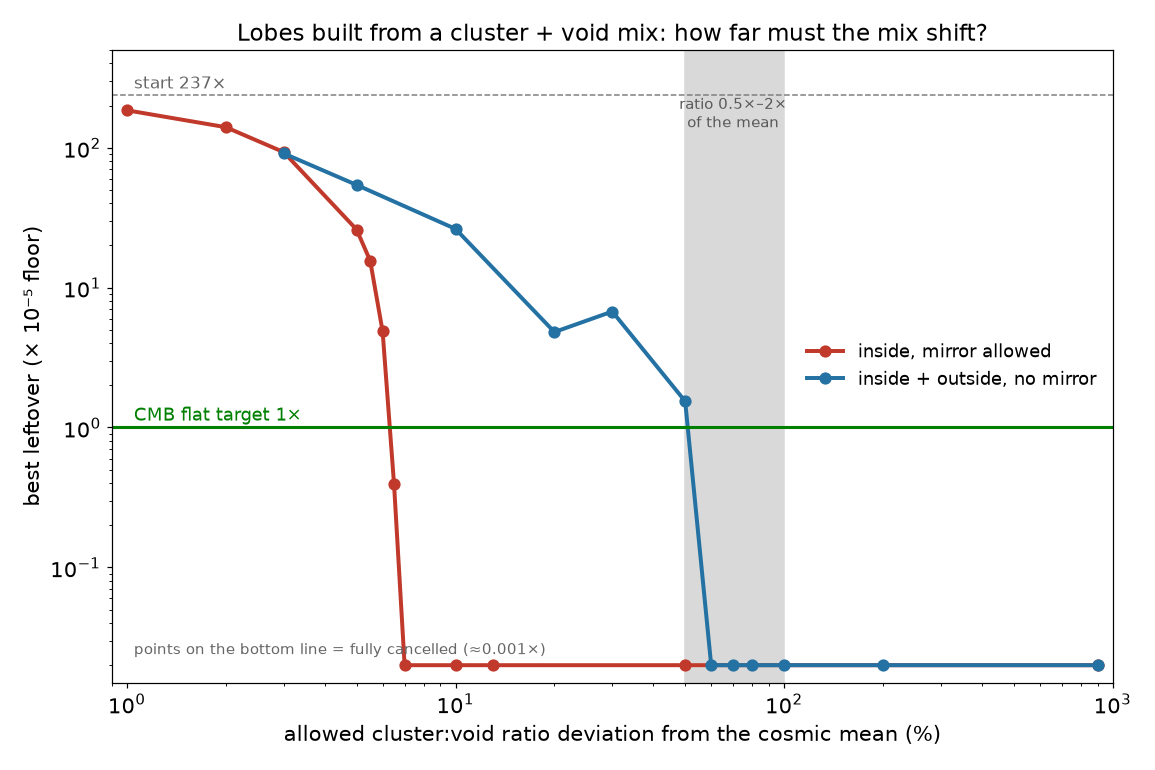
\includegraphics[width=\textwidth]{figures/fig9b_mixed_ratio.png}\caption{}\end{subfigure}
\caption{(a) Number of extra rich clusters and voids that each $1\times$ field corresponds to, compared with how many each region holds anyway. (b) Leftover against how far the local cluster-to-void ratio may differ from the cosmic mean; inside our sphere about $\pm6.5\%$ suffices. The no-mirror curve comes from a solver that stalled and overstates the cost; the converged no-mirror value is about 1.6 times the inside contrast (Sec.~\ref{sec:patch}).}
\label{fig:counts}
\end{figure*}
\begin{figure*}[p]
\centering
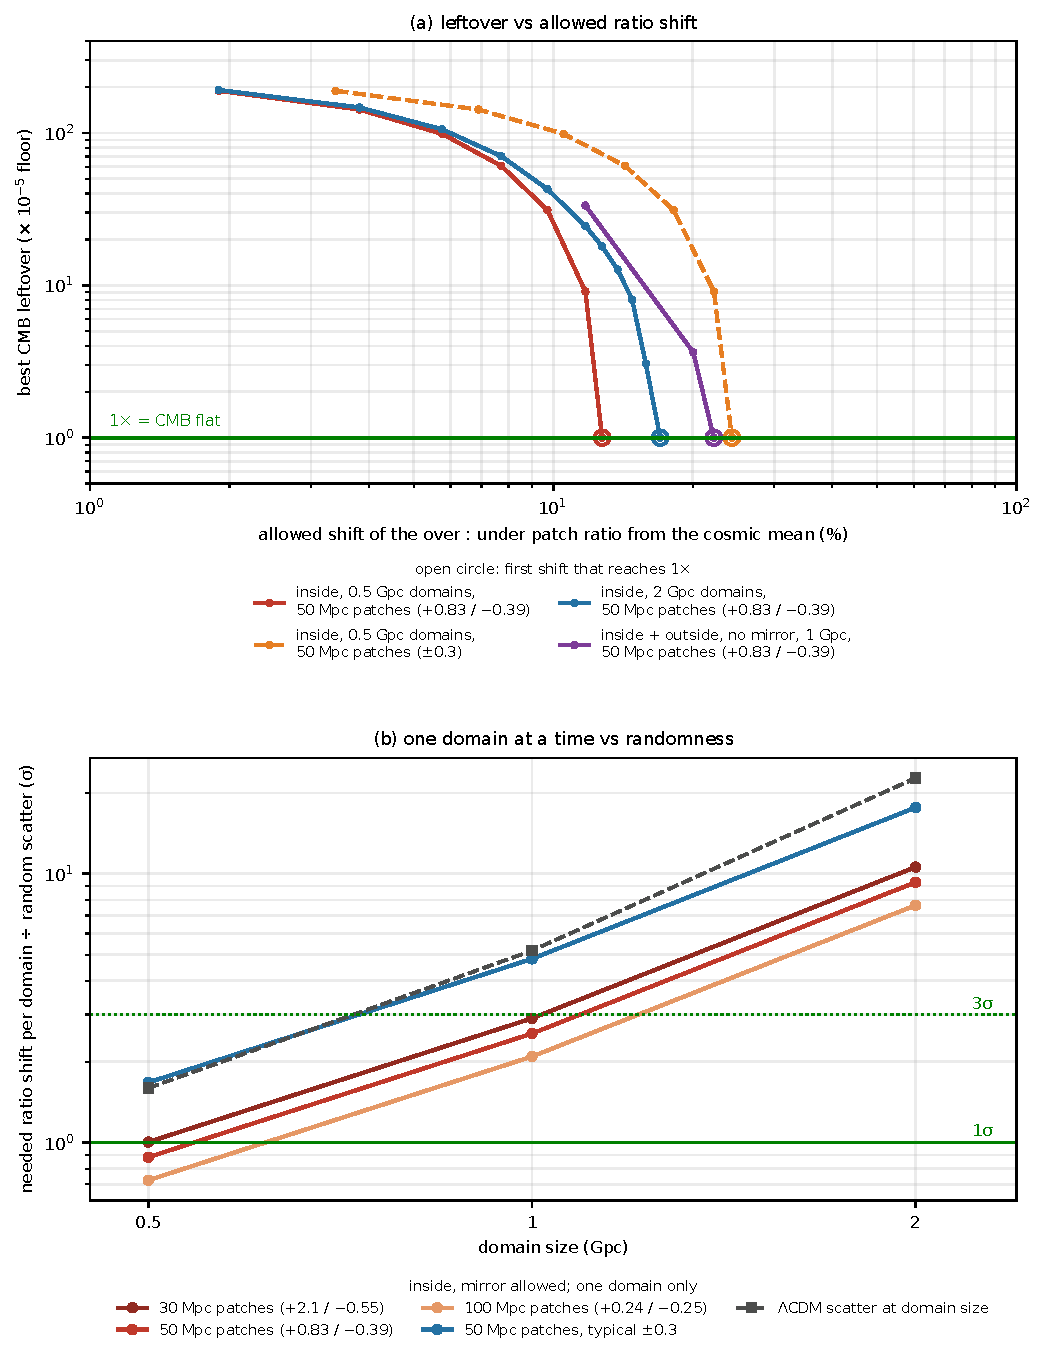
\includegraphics[width=\textwidth,height=0.8\textheight,keepaspectratio]{figures/fig_patch_ratio.pdf}
\caption{Domains built from a fine mix of over- and underdense patches. (a, top) Best leftover against how far the over:under patch ratio of each domain may move from the cosmic mean. Open circles mark the first shift that reaches $1\times$: $+12.7\%$ / $-11.8\%$ for \SI{0.5}{\Gpc} domains and observed-extreme \SI{50}{\Mpc} patches, $+17\%$ / $-15\%$ for \SI{2}{\Gpc} domains, about $+24\%$ for typical $\pm0.3$ patches, and $+22\%$ / $-19\%$ with mirror layouts forbidden (\SI{1}{\Gpc} domains). (b, bottom) The required shift in one domain divided by the random scatter of that domain's patch count, inside our sphere with mirror layouts allowed. This counts one domain only; the coherence over thousands of domains is not included.}
\label{fig:patch}
\end{figure*}
\begin{figure}[tp]
\centering
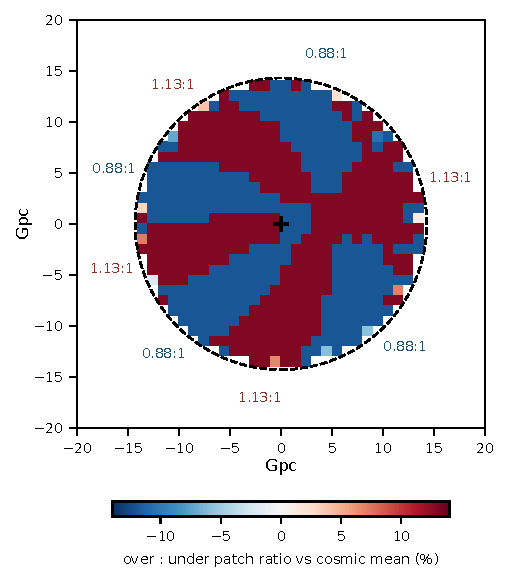
\includegraphics[width=\columnwidth]{figures/fig_patch_map.pdf}
\caption{The required over:under patch ratio, side view (the plane of the CMB ring, seen face-on; dashed: the ring), for \SI{1}{\Gpc} domains and \SI{50}{\Mpc} patches, as a percentage of the cosmic mean. Labels give each lobe's mean ratio relative to the mean. Every domain sits at the allowed limit, in the same eight lobes as the smooth field.}
\label{fig:patchmap}
\end{figure}
\subsection{Example universes and what is left}\label{sec:examples}
Figures~\ref{fig:ex1}--\ref{fig:ex3} show one representative layout per scenario, nine in all, numbered 1--9 from the largest to the smallest leftover; Fig.~\ref{fig:ex4} continues with examples 10--13, the core-open reruns (Sec.~\ref{sec:coreopen}), again from largest to smallest. Each is shown at the first $N$ that reaches $1\times$ (or the best $N$ otherwise), with the mode-by-mode leftover and the residual that remains around the ring. The starting residual is not repeated; it is in Fig.~\ref{fig:fp}. Two patterns recur. The successful fits remove $m=3$--5 almost completely (by factors of $10^4$), and what remains is spread over $m\gtrsim8$, often dominated by modes above 12. The remaining residual is also concentrated near $\ell\approx\ang{180}$--\ang{240}, around the CoE direction.




\subsection{Symmetry, walls and partners}
The best unrestricted fits are close to mirror images across the plane through us and the CoE. The old 0.58\fl\ outside layout has five exact mirror pairs and one body on the axis. Forbidding mirror layouts costs one body: the target is reached at $N=12$ (7 masses and 5 voids, 0.73\fl). A stricter rule that forbids mirror angles alone, regardless of distance and size, stalls at 4.5\fl.

Removing the CoE-interior wall gains one body ($N=10$ instead of 11) and lowers the floor at $N=12$ to about 0.07--0.09\fl. Opening our visible sphere as well gains two more ($N=8$). With the no-mirror rule applied at those $N$, the open solutions rise to 0.54\fl\ ($N=11$, no wall) and 3.7\fl\ ($N=8$, all open).

If our own sphere were on average over- or underdense, its net mass would have to sit in giant partner regions. A uniform contrast of our sphere mostly produces an $m=1$ pattern (515\fl\ per unit $\delta_\mathrm{us}$). The best partner fit (2 partners plus 4 masses and 4 voids, $\delta_\mathrm{us}=-0.025$) reaches 1.23\fl; a layout with a giant \SI{9.2}{\Gpc} partner void and $\delta_\mathrm{us}=+0.21$ reaches 1.57\fl. Partners help, but do not beat ordinary bodies.

\subsection{CoE core fully open}\label{sec:coreopen}
We reran the outside, no-mirror, giant-partner and all-open fits with the CoE interior fully open: no wall and no smooth-density mass cap, with the reach extended along every direction to the far side of the core, up to \SI{102}{\Gpc} from us toward $\ell=\ang{195}$. The mass and radius bounds are unchanged, and of the 214 fits, many started with a third, half or all of their bodies inside the core (Fig.~\ref{fig:coreopen}, examples 10--13 in Fig.~\ref{fig:ex4}). Outside our sphere the target is now reached at $N=10$ (0.46\fl) and the leftover falls to 0.069\fl\ at $N=12$; the no-mirror fits reach it at $N=11$ (0.37\fl), and giant partners plus ordinary bodies reach it for the first time, at $N=10$ (0.17\fl). The all-open result is unchanged: 0.18\fl\ with 8 bodies, as in the earlier all-open run without the density limit, and none of them in the core. Almost all of this gain was already present with the wall removed at the old \SI{43}{\Gpc} reach (0.46, 0.25 and 0.074\fl\ at $N=10$, 11 and 12).

The fits use the core, but only its near edge. Bodies settle a median 3--6\,Gpc inside the edge, about \SI{25}{\Gpc} from us around $\ell\approx\ang{195}$; core-seeded starts move their bodies back out to the edge or leave them parked where they do nothing. With every body forced into the core, the leftover never drops below 143\fl\ (12 bodies). The reason is how fast the needed pull fades with distance. The ring responds to how much a body's pull changes across it, so a distant body pulls almost uniformly and leaves mainly a weak two-lobed ($m=2$) stretch. Table~\ref{tab:coredist} gives the pattern of one \SI{2e52}{\kilo\gram} mass on the us--CoE line: from \SI{20}{\Gpc} to the CoE at \SI{60}{\Gpc} the $m=3$--5 modes, which must cancel 200, 185 and 173\fl, weaken by a factor of 100--1000.

\begin{table}[tbp]
\caption{Ring pattern of one \SI{2e52}{\kilo\gram} mass on the us--CoE line, by mode (units of the floor). The fingerprint's $m=3$, 4, 5 amplitudes are 200, 185 and 173\fl.}
\label{tab:coredist}
\footnotesize
\begin{ruledtabular}
\begin{tabular}{lccc}
distance from us & $m=3$ & $m=4$ & $m=5$\\
\midrule
\SI{20}{\Gpc} (near edge of the core) & 862 & 691 & 541\\
\SI{60}{\Gpc} (at the CoE) & 6.4 & 1.8 & 0.47\\
\SI{100}{\Gpc} (far edge of the core) & 0.81 & 0.13 & 0.02\\
\end{tabular}
\end{ruledtabular}
\end{table}

\subsection{Field solutions}\label{sec:fields}
Instead of individual bodies, one can solve directly for a smooth density contrast $\delta(\mathbf{x})$ inside our sphere with zero net mass (Fig.~\ref{fig:smooth}). The smallest such field that reaches $1\times$ has an rms contrast of 1.0--1.4\% and peaks of 5--7\%, depending on the smoothing scale (1--\SI{4}{\Gpc}); it moves only \SIrange{2e51}{5e51}{\kilo\gram}. It sits just inside the ring and alternates in eight lobes, the same $m=3$--5 pattern turned inside out: an inside deficit acts like an outside excess. The leftover falls from 237\fl\ to 1\fl\ over a narrow range of field strength (Fig.~\ref{fig:smooth}b).

Translated into real objects (Fig.~\ref{fig:counts}a), these fields correspond to a rearrangement of very many ordinary clusters and voids rather than a few giant bodies. If every lobe must be built from a mix of clusters and voids, the local cluster-to-void ratio must differ from the cosmic mean by about $\pm6.5\%$ inside our sphere, (Fig.~\ref{fig:counts}b). Forbidding mirror layouts raises the required contrast to about 1.6 times the inside value (Sec.~\ref{sec:patch}). An earlier no-mirror run, shown in Fig.~\ref{fig:counts}b, suggested 20--60\%, but its solver stalled before converging; that curve is superseded.



\subsection{Over:under patch ratio}\label{sec:patch}
Real domains are not purely over- or underdense; each is a fine mix of small overdense and underdense patches. We therefore let every domain (\SIrange{0.5}{2}{\Gpc}) consist of patches of fixed contrast and vary only the volume fraction of overdense patches, so a domain's net contrast is set by its over:under patch ratio. With \SI{50}{\Mpc} patches at the observed extreme contrasts ($+0.83$ and $-0.39$), the cosmic mean ratio is 0.47:1. Solving for the residual with modes $m=1$--12 (the box-constrained problem solved exactly through its dual), each 0.5--\SI{1}{\Gpc} domain needs only about a $\pm12$--13\% shift in its over:under ratio to reach $1\times$ (Fig.~\ref{fig:patch}a); typical $\pm0.3$ patches need about twice that, and forbidding mirror layouts raises it to about $\pm20\%$ (1.6 times the inside contrast).

Taken one domain at a time, that shift is ordinary: it is about 1--2$\sigma$ of the random scatter in the number of patches per domain ($0.9\sigma$ for \SI{0.5}{\Gpc} domains, $2.6\sigma$ for \SI{1}{\Gpc} domains) (Fig.~\ref{fig:patch}b). The difficulty is coherence. Thousands of domains must all shift the same way, in the same eight lobes, with the $m=3$--5 pattern of the smooth field (Fig.~\ref{fig:patchmap}): ratios of 1.13:1 and 0.88:1 relative to the mean, alternating around the ring and organised over about \SI{5}{\Gpc}. Random patch placement, propagated through the same kernel, produces only 1/6 to 1/13 of the needed CMB pattern, and a $\Lambda$CDM density field about 1/20. The needed pattern is therefore far beyond chance (formally 40--130$\sigma$; these numbers mean ``not by chance'' rather than a precise probability).

\section{Comparison with observed structure}
How unusual would the required structure be? Figure~\ref{fig:dvs} compares the density contrast of the most extreme observed over- and underdense regions with their size: rich clusters \cite{Tinker2008,Rykoff2014,Simet2017}, superclusters \cite{Liivamagi2012}, voids \cite{ClampittJain2015,Mao2017,Hamaus2014}, the Eridanus supervoid behind the Cold Spot \cite{Szapudi2015,Kovacs2016}, the disputed local hole \cite{Keenan2013,Whitbourn2014,Kenworthy2019}, and the densest and emptiest spheres in the 2M++ reconstruction \cite{Carrick2015}. Overdense extremes fall roughly as $|\delta|\propto R^{-1.8}$; at \SI{1}{\Gpc} the required peak contrast is about 19 times the fitted trend of observed extremes. Typical regions (Fig.~\ref{fig:dist}) are far narrower than the extremes: the 2M++ spread falls as $\sigma\approx8.6\,(R/\si{\Mpc})^{-1.0}$ over \SIrange{20}{80}{\Mpc}, and nothing in any catalog reaches \SI{1}{\Gpc}. The homogeneity scale is about \SI{100}{\Mpc} \cite{Scrimgeour2012}; the quasar dipole \cite{Secrest2021} and the cluster anisotropy toward $\ell\approx\ang{280}$ \cite{Migkas2020} are the strongest observed hints of Gpc-scale variation.

\begin{figure*}[tp]
\centering
\begin{subfigure}[b]{0.5\textwidth}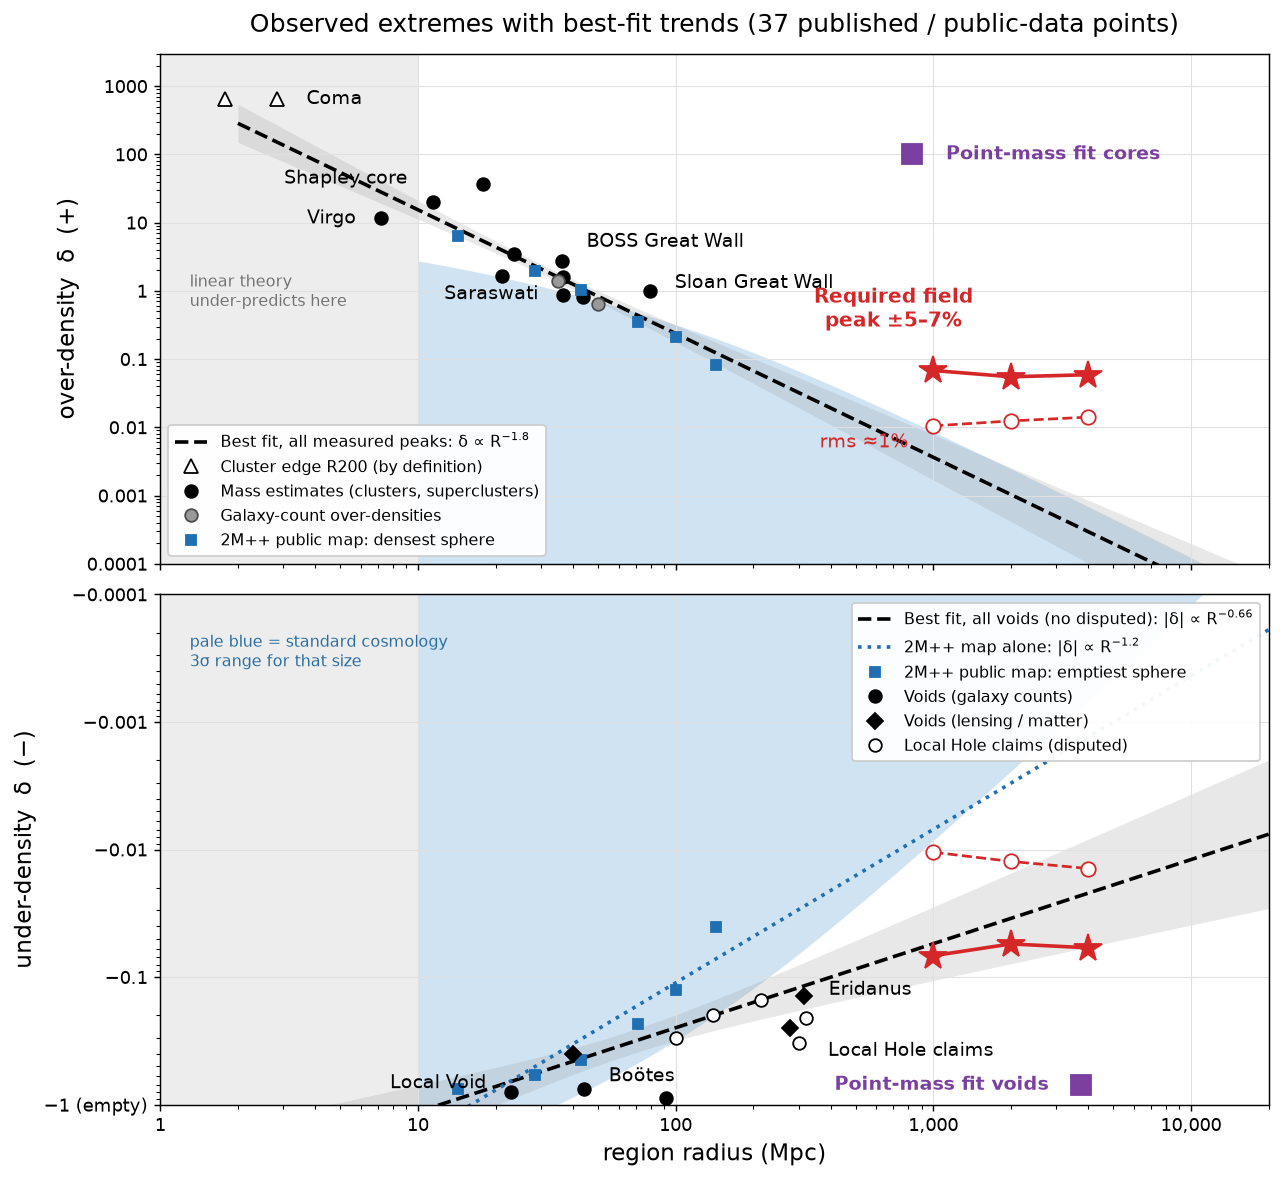
\includegraphics[width=\textwidth]{figures/fig10_density_vs_scale_v2.png}\caption{}\label{fig:dvs}\end{subfigure}\hfill
\begin{subfigure}[b]{0.46\textwidth}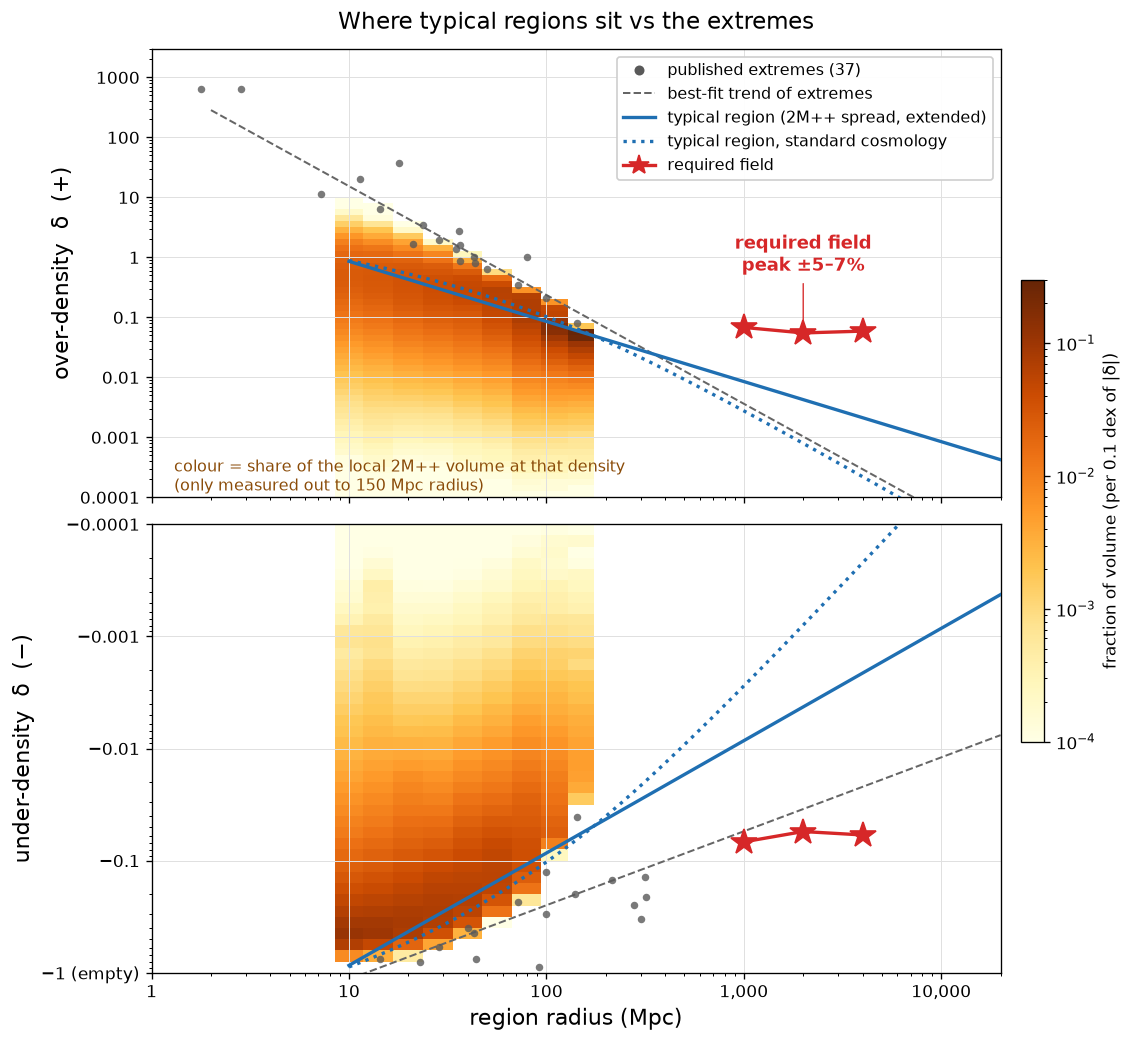
\includegraphics[width=\textwidth]{figures/fig11a_heatmap.png}\caption{}\end{subfigure}
\caption{(a) Density contrast of the most extreme observed regions against their radius, with power-law fits, the standard-cosmology band and the required model markers. (b) The same axes with typical regions (2M++) as a heat map under the extremes.}
\label{fig:dist}
\end{figure*}

\begin{figure*}[tp]
\centering
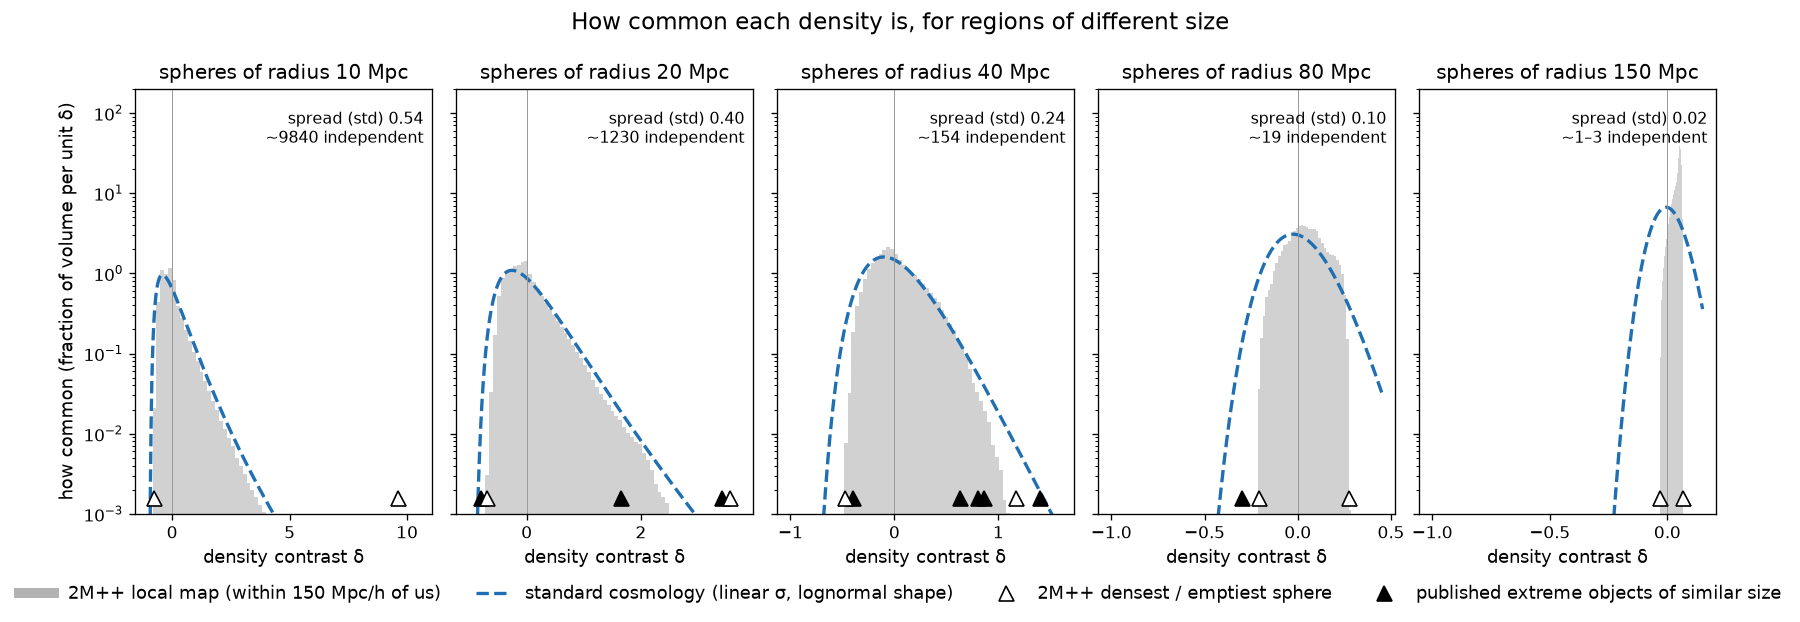
\includegraphics[width=\textwidth]{figures/fig11b_hist.png}
\caption{How common each density contrast is, for 2M++ spheres of 10 to \SI{150}{\Mpc}. The distribution narrows and becomes symmetric as the spheres grow.}
\label{fig:hist}
\end{figure*}

Table~\ref{tab:rare} gives the rarity of the required peak contrast if Gaussian statistics hold at Gpc scales. Even with the generous width extrapolated from 2M++, the \SI{1}{\Gpc} field is an $8\sigma$ event; against linear $\Lambda$CDM \cite{EisensteinHu1998} it is $25\sigma$ or more.

\begin{table}[tbp]
\caption{Rarity of the required peak contrast $|\delta|$ for one region of radius $R$. ``2M++ trend'' extrapolates the observed spread; $\Lambda$CDM uses linear theory at $z=0$.}
\label{tab:rare}
\footnotesize
\begin{ruledtabular}
\begin{tabular}{lcccc}
$R$ & peak $|\delta|$ & width used & $\sigma$ & peak in $\sigma$\\
\midrule
\SI{1}{\Gpc} & 0.068 & 2M++ trend & 0.0085 & 8.0 (6.0--10.5)\\
\SI{1}{\Gpc} & 0.068 & $\Lambda$CDM & 0.0028 & 24.5\\
\SI{2}{\Gpc} & 0.055 & 2M++ trend & 0.0043 & 12.9\\
\SI{2}{\Gpc} & 0.055 & $\Lambda$CDM & 0.00079 & 69\\
\SI{4}{\Gpc} & 0.059 & 2M++ trend & 0.0021 & 28\\
\SI{4}{\Gpc} & 0.059 & $\Lambda$CDM & 0.00022 & 267\\
\end{tabular}
\end{ruledtabular}
\end{table}

\section{Caveats}
\emph{Missing physics.} The kernel includes only the Newtonian tidal and velocity effect. For bodies between us and the ring, the time-varying potentials crossed by CMB photons (integrated Sachs--Wolfe \cite{SachsWolfe1967} and Rees--Sciama \cite{ReesSciama1968} effects), gravitational lensing of the ring, and the potential difference between the ring and us (Sachs--Wolfe term \cite{SachsWolfe1967}) are left out. For \SIrange{e52}{e53}{\kilo\gram} bodies a few Gpc away they are probably not small, so the inside results describe what the tidal model alone says.

\emph{Overfitting.} Each body adds four parameters, while the ring offers 360 samples dominated by about a dozen modes. Above about five bodies many different layouts fit almost equally well, and successful fits push the error into modes above 12. Reaching $1\times$ with 8--12 bodies is thus partly a statement about the number of free parameters.

\emph{Non-uniqueness.} Below about 5 bodies the answer is nearly unique (a backbone of four masses near \SI{20}{\Gpc} at $\ell\approx\ang{75}/\ang{315}$ and \ang{162}/\ang{228}); beyond that the examples shown are illustrations, not unique answers. The smooth field is the minimum-norm solution; many other fields also work.

\emph{Ring-plane only.} Only the in-plane ring is constrained, so nothing is known about structure far above or below the galactic plane; a full-sky fit would need more structure.

\emph{Extrapolation.} The comparison with observed structure extrapolates the 2M++ spread from \SI{80}{\Mpc} to \SIrange{1}{4}{\Gpc}, a factor of 12--50 in radius, and assumes Gaussian tails.

\emph{Faster-than-light recession.} The model expects the outer parts of the shell to recede faster than light. Spreading the shell's outer edge (\SI{72.5}{\Gpc}) over an age of \SI{13.8}{Gyr} gives an average edge speed of about $17c$ in Newtonian terms; a Sedov--Taylor scaling ($R\propto t^{2/5}$) puts today's edge speed at two fifths of that, about $7c$. This is expected for expanding space: it is a recession velocity, not motion through space, so it does not conflict with relativity, but the Newtonian kernel used here does not treat it. The next stage of model development is a full relativistic Lema\^itre--Tolman--Bondi (LTB) treatment, in which the energy function $E(r)$ must satisfy $2E/c^2>-1$, grow as $E\propto r^2$ near the centre, avoid shell crossing, and match the local Hubble constant $H_0$ where we sit.

\section{Conclusions}
The CoE shell model leaves a specific fingerprint in the CMB ring: a 237\fl\ pattern dominated by three to five waves around the sky. Treated as an inverse problem, this fingerprint can be cancelled to the flat target by a small number of deliberately placed bodies: 11 outside our visible sphere, 4 to 8 inside it, and 8 when no placement wall is imposed. With the CoE core fully open, 10 outside bodies suffice, all within a few Gpc of the core's near edge; the deep core contributes almost nothing because the $m=3$--5 pull fades rapidly with distance. Both masses and voids are needed outside; inside, masses alone suffice. Requiring that the layout not be a mirror image costs about one body.

The solutions are not unique, and above a handful of bodies the fits are as much a measure of freedom as of physics. Sequential growth that never revisits earlier choices fails by a wide margin, which suggests that the cancellation needs coordinated, not accumulated, structure.

The smooth-field solutions show what the cancellation would demand of the real universe: a coherent pattern of about 1\% rms and 5--7\% peaks on gigaparsec scales, arranged in the same three-to-five-lobe shape as the fingerprint. That is about an $8\sigma$ fluctuation at \SI{1}{\Gpc} even against the most generous extrapolation of observed structure. A fuller treatment would add the line-of-sight effects listed above, fit the whole sky rather than the ring alone, and replace the Newtonian kernel with a relativistic LTB model that handles the faster-than-light recession the model expects.


\bibliography{refs}
\end{document}
